\documentclass[
    english,
    ruledheaders=section,
    class=report,
    thesis={type=bachelor},
    accentcolor=2d,
    custommargins=false,
    marginpar=false,
    parskip=half-,
    fontsize=11pt,
    pdfa=false,
]{tudapub}

\usepackage[main=english]{babel}
\usepackage{biblatex}
\usepackage{csquotes}
\addbibresource{thesis.bib}
\usepackage{stmaryrd, amsmath, amssymb, amsfonts, amsthm}
\usepackage{multicol}
\usepackage{mathtools}
\usepackage{bussproofs}
\usepackage{xcolor}
\usepackage{mathrsfs}
\usepackage{xspace}
\usepackage{paralist}
\usepackage{nicefrac}
\usepackage{multirow}
\usepackage{tikz}
\usetikzlibrary{calc,trees,decorations,arrows,automata,positioning,plotmarks, shapes,shapes.geometric,backgrounds}
\newcommand{\TODO}[1]{\textcolor{red}{#1}}
\DeclareUnicodeCharacter{2212}{-}

% \newtheorem{condition}[corollary]{Condition}

%%%%%%%%%%%%%%%%%%%%%%%%%%%%%%%%%
%  abbreviations and key words  %
%%%%%%%%%%%%%%%%%%%%%%%%%%%%%%%%%

% makros for text
\newcommand{\ie}{i.e.,\xspace}
\newcommand{\eg}{e.g.\xspace}
\newcommand{\wrt}{w.r.t.\ }
\newcommand{\cf}{cf.\ }
\newcommand{\MPST}{MPST\xspace}
\newcommand{\piCal}{$ \pi $-calculus\xspace}
\newcommand{\PiCal}{$ \pi $-Calculus\xspace}
\newcommand{\strongR}{strong\-ly re\-li\-ab\-le\xspace}
\newcommand{\StrongR}{Strong\-ly Re\-li\-ab\-le\xspace}
\newcommand{\weakR}{weak\-ly re\-li\-ab\-le\xspace}
\newcommand{\WeakR}{Weak\-ly Re\-li\-ab\-le\xspace}
\newcommand{\unrel}{un\-re\-li\-ab\-le\xspace}
\newcommand{\Unrel}{Un\-re\-li\-ab\-le\xspace}

% makros for formulas
\newcommand{\iR}{\operatorname{r}}
\newcommand{\iU}{\operatorname{u}}
\newcommand{\iW}{\operatorname{w}}
\newcommand{\Set}[2][]{\left\lbrace #1 #2 #1 \right\rbrace}
\newcommand{\nat}{\mathbb{N}}
\newcommand{\deff}{\; \triangleq \;}
\newcommand{\deffTerms}{\; \mathop{::=} \;}
\newcommand{\sepTerms}{\hspace{0.75em} | \hspace{0.75em}}
\newcommand{\logdot}{. \;}
\newcommand{\Subst}[2]{{\Set{ \nicefrac{#1}{#2} }}}
\newcommand{\Length}[1]{\left| #1 \right|}
\newcommand{\indexSet}[1][I]{\mathrm{#1}}

%%%%%%%%%%%%%%%%%%%%%%%%%%%%%%
%  multiparty session types  %
%%%%%%%%%%%%%%%%%%%%%%%%%%%%%%

% names, variables, channels, ...
\newcommand{\default}{\operatorname{d}}
\newcommand{\roles}{\mathcal{R}}
\newcommand{\Role}[1][r]{\mathsf{#1}}
\newcommand{\Roles}[1]{\operatorname{R}\!\left( #1 \right)}
\newcommand{\Actors}[1]{\operatorname{A}\!\left( #1 \right)}
\newcommand{\labels}{\mathcal{L}}
\newcommand{\Label}[1][l]{\mathit{#1}}
\newcommand{\LabelD}{\Label_{\operatorname{d}}}
\newcommand{\LabelB}{\Label_{\operatorname{b}}}
\newcommand{\names}{\mathcal{N}}
\newcommand{\FreeNames}[1]{\operatorname{FN}\!\left( #1 \right)}
\newcommand{\BoundNames}[1]{\operatorname{BN}\!\left( #1 \right)}
\newcommand{\Args}[1][x]{\mathit{#1}}
\newcommand{\Chan}[1][s]{\mathit{#1}}
\newcommand{\typeVars}{\mathcal{V}_{\operatorname{T}}}
\newcommand{\TypeV}[1][t]{\mathit{#1}}
\newcommand{\procVars}{\mathcal{V}_{\operatorname{P}}}
\newcommand{\ProcV}[1][X]{\mathit{#1}}
\newcommand{\atomicTypes}{\mathcal{A}}
\newcommand{\AtomicType}[1]{\mathrm{#1}}
\newcommand{\sorts}{\mathcal{S}}
\newcommand{\Sort}[1][S]{\mathrm{#1}}
\newcommand{\expressions}{\mathcal{E}}
\newcommand{\Expr}[1][e]{#1}
\newcommand{\bool}{\mathbb{B}}
\newcommand{\true}{\mathtt{t}}
\newcommand{\false}{\mathtt{f}}

% global types
\newcommand{\globalTypes}{\mathcal{G}}
\newcommand{\GT}[1][G]{#1}
\newcommand{\GTD}{\GT_{\operatorname{d}}}
\newcommand{\GTB}{\GT_{\operatorname{b}}}
\newcommand{\GComR}[4]{#1 \to_{\iR} #2{:}{\left< #3 \right>}.#4}
\newcommand{\GComU}[5]{#1 \to_{\iU} #2{:}#3{\left< #4 \right>}.#5}
\newcommand{\GComUS}[4]{#1 \to_{\iU} #2{:}#3{\left< #4 \right>}}
\newcommand{\GBranR}[3]{#1 \to_{\iR} #2{:}{#3}}
\newcommand{\GBranW}[3]{#1 \to_{\iW} #2{:}{#3}}
\newcommand{\GPar}[2]{#1 \; || \; #2}
\newcommand{\GRep}[2]{{\left( \mu #1 \right)} #2}
\newcommand{\GEnd}{\mathtt{end}}
\newcommand{\GDel}[6]{#1 \to #2{:}{\left< \Typed{\AT{#3}{#4}}{#5} \right>}.#6}

% local types
\newcommand{\localTypes}{\mathcal{T}}
\newcommand{\LT}[1][T]{#1}
\newcommand{\LTD}{\LT_{\operatorname{d}}}
\newcommand{\LTB}{\LT_{\operatorname{b}}}
\newcommand{\LSendR}[3]{{\left[ #1 \right]}\mathsf{!}_{\iR}{\left< #2 \right>}.#3}
\newcommand{\LGetR}[3]{{\left[ #1 \right]}\mathsf{?}_{\iR}{\left< #2 \right>}.#3}
\newcommand{\LSendU}[4]{{\left[ #1 \right]}\mathsf{!}_{\iU}#2{\left< #3 \right>}.#4}
\newcommand{\LGetU}[4]{{\left[ #1 \right]}\mathsf{?}_{\iU}#2{\left< #3 \right>}.#4}
\newcommand{\LSelR}[2]{{\left[ #1 \right]}\mathsf{!}_{\iR}{#2}}
\newcommand{\LBranR}[2]{{\left[ #1 \right]}\mathsf{?}_{\iR}{#2}}
\newcommand{\LSelW}[2]{{\left[ #1 \right]}\mathsf{!}_{\iW}{#2}}
\newcommand{\LBranW}[2]{{\left[ #1 \right]}\mathsf{?}_{\iW}{#2}}
\newcommand{\LRep}[2]{{\left( \mu #1 \right)} #2}
\newcommand{\LEnd}{\mathtt{end}}
\newcommand{\LDelA}[5]{{\left[ #1 \right]}\mathsf{!}{\left< \Typed{\AT{#2}{#3}}{#4} \right>}.#5}
\newcommand{\LDelB}[5]{{\left[ #1 \right]}\mathsf{?}{\left< \Typed{\AT{#2}{#3}}{#4} \right>}.#5}

% session calculus
\newcommand{\processes}{\mathcal{P}}
\newcommand{\PT}[1][P]{\ensuremath{\mathit{#1}}}
\newcommand{\PTD}[1][P]{\PT[#1]_{\operatorname{d}}}
\newcommand{\PTB}[1][P]{\PT[#1]_{\operatorname{b}}}
\newcommand{\PReq}[4]{\overline{#1}{\left[ #2 \right]}{\left( #3 \right)}.#4}
\newcommand{\PAcc}[4]{#1{\left[ #2 \right]}{\left( #3 \right)}.#4}
\newcommand{\PSendR}[5]{#1{\left[ #2, #3 \right]}\mathsf{!}_{\iR}{\left< #4 \right>}.#5}
\newcommand{\PGetR}[5]{#1{\left[ #2, #3 \right]}\mathsf{?}_{\iR}{\left( #4 \right)}.#5}
\newcommand{\PSendU}[6]{#1{\left[ #2, #3 \right]}\mathsf{!}_{\iU}#4{\left< #5 \right>}.#6}
\newcommand{\PSendUS}[5]{#1{\left[ #2, #3 \right]}\mathsf{!}_{\iU}#4{\left< #5 \right>}}
\newcommand{\PGetU}[7]{#1{\left[ #2, #3 \right]}\mathsf{?}_{\iU}#4{\left< #5 \right>}{\left( #6 \right)}.#7}
\newcommand{\PGetUS}[6]{#1{\left[ #2, #3 \right]}\mathsf{?}_{\iU}#4{\left< #5 \right>}{\left( #6 \right)}}
\newcommand{\PSelR}[5]{#1{\left[ #2, #3 \right]}\mathsf{!}_{\iR}#4.#5}
\newcommand{\PBranR}[4]{#1{\left[ #2, #3 \right]}\mathsf{?}_{\iR}{#4}}
\newcommand{\PSelW}[5]{#1{\left[ #2, #3 \right]}\mathsf{!}_{\iW}#4.#5}
\newcommand{\PSelWS}[4]{#1{\left[ #2, #3 \right]}\mathsf{!}_{\iW}#4}
\newcommand{\PBranW}[4]{#1{\left[ #2, #3 \right]}\mathsf{?}_{\iW}{#4}}
\newcommand{\myif}{\mathtt{if}}
\newcommand{\mythen}{\mathtt{then}}
\newcommand{\myelse}{\mathtt{else}}
\newcommand{\PITE}[3]{\myif \; #1 \; \mythen \; #2 \; \myelse \; #3}
\newcommand{\PPar}[2]{#1 \mid #2}
\newcommand{\PDelA}[5]{#1{\left[ #2, #3 \right]}\mathsf{!}{\left<\!{\left< #4 \right>}\!\right>}.#5}
\newcommand{\PDelB}[5]{#1{\left[ #2, #3 \right]}\mathsf{?}{\left(\!{\left( #4 \right)}\!\right)}.#5}
\newcommand{\PRes}[2]{{\left( \nu #1 \right)} #2}
\newcommand{\PRep}[2]{{\left( \mu #1 \right)} #2}
\newcommand{\PEnd}{\mathbf{0}}
\newcommand{\PCrash}{\bot}
\newcommand{\Queue}[1][M]{\mathrm{#1}}
\newcommand{\MQ}[4]{#1_{#2 \to #3}{:}#4}
\newcommand{\MQS}[3]{#1_{#2 \to #3}}
\newcommand{\emptyList}{[\,]}

% semantics of processes
\newcommand{\step}{\longmapsto}
\newcommand{\steps}{\longmapsto^*}
\newcommand{\stepsP}{\longmapsto^+}
\newcommand{\nStep}{\; \not\!\!\longmapsto}
\newcommand{\compL}[1][\;]{#1\dot{=}#1}
\newcommand{\nCompL}[1][\;]{#1\not\!\!\dot{=}#1}
\newcommand{\Eval}[1]{{\operatorname{eval}}{\left( #1 \right)}}
\newcommand{\fpUGet}{\mathtt{FP}_{\mathtt{uget}}}
\newcommand{\fpUSkip}{\mathtt{FP}_{\mathtt{uskip}}}
\newcommand{\fpML}{\mathtt{FP}_{\mathtt{ml}}}
\newcommand{\fpWSkip}{\mathtt{FP}_{\mathtt{wskip}}}
\newcommand{\fpCrash}{\mathtt{FP}_{\mathtt{crash}}}

% messages
\newcommand{\messages}{\mathcal{M}}
\newcommand{\messageTypes}{\mathcal{MT}}
\newcommand{\MT}[1][MT]{\mathrm{#1}}
\newcommand{\MessR}[1]{{\left< #1 \right>^{\iR}}}
\newcommand{\MessU}[2]{#1{\left< #2 \right>^{\iU}}}
\newcommand{\MessBR}[1]{#1^{\iR}}
\newcommand{\MessBW}[1]{#1^{\iW}}

% well-typedness
\newcommand{\AT}[2]{#1{\left[ #2 \right]}}
\newcommand{\Typed}[2]{#1{:}#2}
\newcommand{\compS}{\cdot}
\newcommand{\Proj}[2]{{#1}{\restriction_{#2}}}
\newcommand{\Unreliable}[1]{{\operatorname{nsr}}{\left( #1 \right)}}

%%%%%%%%%%%%%%
%  Examples  %
%%%%%%%%%%%%%%

% example to explain the syntax
\newcommand{\GDice}{\GT_{\text{dice}, \iR}}
\newcommand{\GDiceUC}{\GT_{\text{dice}, \iU}}
\newcommand{\GDiceW}{\GT_{\text{dice}}}
\newcommand{\LDice}[1]{\LT_{\Role[#1]:\text{dice}, \iR}}
\newcommand{\LDiceW}[1]{\LT_{\Role[#1]:\text{dice}}}
\newcommand{\PDice}{\PT_{\text{dice}}}
\newcommand{\PDiceD}{\PT_{\Role[3]}}
\newcommand{\PDiceP}{\PT_{\Role[i]}}
\newcommand{\PDiceQ}{\PT_{\Role[2]}}
\newcommand{\PDiceR}{\PT_{\Role[1]}}
\newcommand{\PDiceUC}{\PT_{\text{dice}, \iU}}
\newcommand{\PDiceDUC}{\PT_{\Role[3], \iU}}
\newcommand{\PDicePUC}{\PT_{\Role[i], \iU}}
\newcommand{\PDiceQUC}{\PT_{\Role[2], \iU}}

% large example
\newcommand{\GTLE}[2][G]{\GT[#1]_{\operatorname{sub}}\!\left( #2 \right)}
\newcommand{\GTLEC}[2][G]{\GT[#1]_{\operatorname{ct}}\!\left( #2 \right)}
\newcommand{\SortBel}{\ensuremath{\Sort_{\mathrm{belief}}}}
\newcommand{\SortAck}{\ensuremath{\Sort_{\mathrm{ack}}}}
\newcommand{\RCSys}{\PT[Sys]\!\left( \Role[n], \InitKnowledge \right)}
%\newcommand{\RCP}[3][P]{\PT[#1]_{\operatorname{p_{1}}}\!\left( #2, #3 \right)}
\newcommand{\RCP}[2][i]{\PT[P]\!\left( \Role[#1], \Role[n], #2  \right)}
\newcommand{\RCPe}[2][i]{\PT[P]\!\left( #1, \Role[3], #2  \right)}
\newcommand{\RCPi}{\PT[P]_{\operatorname{1}}\!\left( \Role[i], \Role[n], r, \Knowledge \right)}
\newcommand{\RCPio}[2][C]{\PT[P]_{\operatorname{1}}^{\operatorname{#1}}\!\left( \Role[#2], \Role[n], \Role[c], \Knowledge \right)}
\newcommand{\RCPioe}[4][C]{\PT[P]_{\operatorname{1}}^{\operatorname{#1}}\!\left( #2, \Role[3], #3, #4 \right)}
\newcommand{\RCPiio}[3][C]{\PT[P]_{\operatorname{2}}^{\operatorname{#1}}\!\left( \Role[#2], \Role[n], \Role[c], #3 \right)}
\newcommand{\RCPiioe}[4][C]{\PT[P]_{\operatorname{2}}^{\operatorname{#1}}\!\left( #2, \Role[3], #3, #4 \right)}
\newcommand{\RCPiiio}[2][C]{\PT[P]_{\operatorname{3}}^{\operatorname{#1}}\!\left( \Role[#2], \Role[n], \Role[c], \Knowledge \right)}
\newcommand{\RCPiiioe}[4][C]{\PT[P]_{\operatorname{3}}^{\operatorname{#1}}\!\left( #2, \Role[3], #3, #4 \right)}
\newcommand{\RCPiiin}[4][NC]{\PT[P]_{\operatorname{3}}^{\operatorname{#1}}\!\left( \Role[#2], \Role[n], \Role[c], #3, #4 \right)}
\newcommand{\RCPiiine}[5][NC]{\PT[P]_{\operatorname{3}}^{\operatorname{#1}}\!\left( #2, \Role[3], #3, #4, #5 \right)}
\newcommand{\RCPiv}{\PT[P]_{\operatorname{4}}\!\left( \Role[i], \Role[n], r, \Knowledge \right)}
\newcommand{\RCPive}[3]{\PT[P]_{\operatorname{4}}\!\left( #1, \Role[3], #2, #3 \right)}
\newcommand{\RCPivo}[2][C]{\PT[P]_{\operatorname{4}}^{\operatorname{#1}}\!\left( \Role[#2], \Role[n], \Role[c], \Knowledge \right)}
\newcommand{\RCPivoe}[4][C]{\PT[P]_{\operatorname{4}}^{\operatorname{#1}}\!\left( #2, \Role[3], #3, #4 \right)}
\newcommand{\InitKnowledge}[1][]{\ensuremath{\vec{V^{0}_{\Role[#1]}}}} % todo, sieht scheiße aus
\newcommand{\Knowledge}{\ensuremath{\vec{V}}} %todo
\newcommand{\KnowledgeE}[2][]{\ensuremath{\vec{V_{#2}^{#1}}}}
\newcommand{\FuncBest}{\ensuremath{\operatorname{best}}}
\newcommand{\FuncReceived}{\ensuremath{\operatorname{received}}}
\newcommand{\FuncCountAck}{\ensuremath{\operatorname{ack}}}
\newcommand{\FuncUpdate}{\ensuremath{\operatorname{update}}}
\newcommand{\ceilTwo}[1]{\ensuremath{\bigg\lceil#1\bigg\rceil}}
\newcommand{\FDS}{\ensuremath{\Diamond \mathcal{S}}\xspace}
\newcommand{\PTMQ}[1][P]{\ensuremath{\PT[#1]_{\mathit{MQ}}}}
\newcommand{\ATE}[2]{\AT[]{\Chan[#1]\!}{\Role[#2]}}
\newcommand{\ImplMajor}{\ensuremath{\big\lceil\frac{\Role[n]-1}{2}\big\rceil}\xspace}

\newtheoremstyle{paxos}{}{}{\itshape}{}{\bfseries}{}{.5em}{\thmnote{#3}}
\theoremstyle{paxos}
\newtheorem*{paxostheoremenv}{}
\newtheorem*{reductionrule}{}

\theoremstyle{definition}
\newtheorem{phase}{Phase}
\newtheorem*{assumption}{Assumption}
\newtheorem*{asyncdef}{Definition}
\newtheorem{algorithmdef}{A}

\newcommand{\PaxosTheoremConstructor}[2]{\operatorname{P#1^{#2}}}
\newcommand{\PaxosTheorem}[1]{\PaxosTheoremConstructor{#1}{}}
\newcommand{\PaxosSubtheorem}[2]{\PaxosTheoremConstructor{#1}{#2}}

% General typesetting stuff
\newcommand{\Curly}[1]{\left\{#1\right\}}
\newcommand{\Paren}[1]{\left(#1\right)}
\newcommand{\Bracket}[1]{\left[#1\right]}
\newcommand{\comment}[1]{\;\textcolor{teal}{#1}}
\def\IndentationSize{0.75em}
\newcommand{\Indent}[1]{\hspace*{\IndentationSize * #1}}

% Technical Preliminaries
\newcommand{\FTMPST}[0]{FTMPST\xspace}

% Sorts
\newcommand{\Bool}[0]{\operatorname{Bool}}
\newcommand{\True}[0]{\operatorname{true}}
\newcommand{\False}[0]{\operatorname{false}}
\newcommand{\Maybe}[1]{\operatorname{Maybe}\; #1}
\newcommand{\Just}[1]{\operatorname{Just}\; #1}
\newcommand{\Nothing}[0]{\operatorname{Nothing}}
\newcommand{\Or}[0]{\; | \;}
\newcommand{\Promise}[1]{\operatorname{Promise}\; #1}
\newcommand{\Proposal}[1]{\operatorname{Proposal}\; #1}
\newcommand{\ProposalC}[2]{\operatorname{Proposal}\; #1\; #2}
\newcommand{\Nack}[1]{\operatorname{Nack}\; #1}
\newcommand{\Value}[0]{\operatorname{Value}}
\newcommand{\TypeParamA}[0]{\ensuremath{\operatorname{a}}\xspace}
\newcommand{\TypeParamB}[0]{\ensuremath{\operatorname{b}}\xspace}
\newcommand{\Sab}[0]{\ensuremath{\operatorname{S}\;\TypeParamA\;\TypeParamB}\xspace}
\newcommand{\Scd}[0]{\ensuremath{\operatorname{S}\;\operatorname{c}\;\operatorname{d}}\xspace}

% MPST
%% General
\newcommand{\DotForall}[2]{\textstyle\left(\bigodot_{#1}\;#2\right)}
\newcommand{\Mu}[1]{\left(\mu #1\right)}
\newcommand{\AQ}[0]{\operatorname{Q}}
\newcommand{\QRoles}[0]{\operatorname{R}}
\newcommand{\End}[0]{0}

%% Phases
\newcommand{\POneA}[0]{1a}
\newcommand{\POneB}[0]{1b}
\newcommand{\PTwoA}[0]{2a}
\newcommand{\PTwoB}[0]{2b}
\newcommand{\LOneA}[0]{l1a}
\newcommand{\LOneB}[0]{l1b}
\newcommand{\LTwoA}[0]{l2a}
\newcommand{\LTwoB}[0]{l2b}

%% Global Type
\newcommand{\ProposerRole}[0]{p}
\newcommand{\AcceptorRole}[0]{a}
\newcommand{\OuterSharedPoint}[0]{o}
\newcommand{\SharedPoint}[1]{b_{#1}}
\newcommand{\OuterSessionChannel}[0]{z}
\newcommand{\SessionChannel}[0]{s}
\newcommand{\OuterGlobalType}[0]{\operatorname{G}}
\newcommand{\GlobalType}[0]{\operatorname{G_{\ProposerRole, A_Q}}}
\newcommand{\SendUnreliableG}[4]{#1 \to_u #2 : #3 \left\langle #4 \right\rangle}
\newcommand{\SendWeaklyG}[3]{#1 \to_w #2 : \Curly{#3}}
\newcommand{\RecursionVariableType}[0]{t}

%% Local Type
\newcommand{\SendUnreliableL}[3]{\left[#1\right]!_u #2 \left\langle #3 \right\rangle}
\newcommand{\ReceiveUnreliableL}[3]{\left[#1\right]?_u #2 \left\langle #3 \right\rangle}
\newcommand{\SendWeaklyL}[2]{\left[#1\right]!_w \Curly{#2}}
\newcommand{\ReceiveWeaklyL}[3]{\left[#1\right]?_w \Curly{#2}_{#3}}
\newcommand{\OuterGlobalTypeProjection}[1]{\OuterGlobalType \upharpoonright_{#1}}
\newcommand{\GlobalTypeProjection}[1]{\GlobalType \upharpoonright_{#1}}

%% Process
\newcommand{\SendUnreliableP}[5]{#1\left[#2, #3\right]!_u #4 \left\langle #5 \right\rangle}
\newcommand{\ReceiveUnreliableP}[6]{#1\left[#2, #3\right]?_u #4 \left\langle #5 \right\rangle \left(#6\right)}
\newcommand{\SendWeaklyP}[5]{#1\left[#2, #3\right]!_w #4.#5}
\newcommand{\ReceiveWeaklyP}[4]{#1\left[#2, #3\right]?_w \big\{#4\big\}}
\newcommand{\RecursionVariable}[0]{X}

% Failure Patterns
\newcommand{\FPuget}[0]{\mathtt{FP_{uget}}}
\newcommand{\FPuskip}[0]{\mathtt{FP_{uskip}}}
\newcommand{\FPml}[0]{\mathtt{FP_{ml}}}
\newcommand{\FPwskip}[0]{\mathtt{FP_{wskip}}}
\newcommand{\FPcrash}[0]{\mathtt{FP_{crash}}}
\newcommand{\FailureDetectorClass}[0]{\Diamond\mathscr{S}}

% Paxos Process
\newcommand{\Call}[2]{#1\left(#2\right)}
\newcommand{\AcceptorCount}[0]{c_A}
\newcommand{\ProposerCount}[0]{c_P}
\newcommand{\Accept}[0]{\mathnormal{Accept}}
\newcommand{\Restart}[0]{\mathnormal{Restart}}
\newcommand{\Abort}[0]{\mathnormal{Abort}}
\newcommand{\Sys}[2]{\operatorname{Sys}\left(#1, #2\right)}
\newcommand{\Process}[2]{\operatorname{P^{#1}_{#2}}}
\newcommand{\Pa}[1]{\Process{A}{#1}}
\newcommand{\Pp}[1]{\Process{P}{}\left(#1\right)}
\newcommand{\PaOne}[0]{\Pa{1}}
\newcommand{\PaTwo}[0]{\Pa{2}}
\newcommand{\PaAccept}[0]{\Pa{acc}}
\newcommand{\PpInitName}[0]{\Process{P}{init}}
\newcommand{\PpInit}[1]{\textstyle\PpInitName\left(#1\right)}
\newcommand{\PpInitShort}[0]{\PpInitName\left(\dots\right)}
\newcommand{\PaInitName}[0]{\Pa{init}}
\newcommand{\PaInit}[1]{\PaInitName\left(#1\right)}
\newcommand{\PaInitShort}[0]{\PaInitName\left(\dots\right)}
\newcommand{\SessionRequest}[3]{\overline{#1}\left[#2\right]\left(#3\right)}
\newcommand{\SessionAccept}[3]{#1\left[#2\right]\left(#3\right)}
\newcommand{\ParallelFor}[1]{\Pi_{#1}\;}
\newcommand{\Acceptor}[1]{\ensuremath{\operatorname{A_{#1}}}}
\newcommand{\Proposer}[1]{\ensuremath{\operatorname{P_{#1}}}}

% Functions
\newcommand{\proposalNumberName}[0]{\operatorname{proposalNumber}}
\newcommand{\proposalNumber}[2]{\proposalNumberName_#2\left( #1\right)}

\newcommand{\promiseValueName}[0]{\operatorname{promiseValue}}
\newcommand{\promiseValue}[1]{\promiseValueName\left(#1\right)}

\newcommand{\anyNackName}[0]{\operatorname{anyNack}}
\newcommand{\anyNack}[1]{\anyNackName\left(#1\right)}

\newcommand{\promiseCountName}[0]{\operatorname{promiseCount}}
\newcommand{\promiseCount}[1]{\promiseCountName\left(#1\right)}

\newcommand{\greaterThanName}[0]{\operatorname{gt}}
\newcommand{\greaterThan}[2]{\greaterThanName\left(#1, #2\right)}

\newcommand{\greaterEqualName}[0]{\operatorname{ge}}
\newcommand{\greaterEqual}[2]{\greaterEqualName\left(#1, #2\right)}

\newcommand{\nFromProposalName}[0]{\operatorname{nFromProposal}}
\newcommand{\nFromProposal}[1]{\nFromProposalName\left(#1 \right)}

\newcommand{\genAqName}[0]{\operatorname{gen\AQ}}
\newcommand{\genAq}[3]{\genAqName\left(#1, #2, #3\right)}

\newcommand{\positionHelperName}[0]{\operatorname{positionHelper}}
\newcommand{\positionHelper}[3]{\positionHelperName\left(#1, #2, #3\right)}

\newcommand{\positionName}[0]{\operatorname{position}}
\newcommand{\position}[2]{\positionName\left(#1, #2\right)}

\newcommand{\update}[2]{\operatorname{update} \left(#1, #2\right)}

% Math and Programming
\newcommand{\ceil}[1]{\Big\lceil #1 \Big\rceil}
\newcommand{\VectorV}[0]{\overrightarrow{V}}
\newcommand{\If}[1]{\operatorname{if}\xspace #1}
\newcommand{\Then}[1]{\operatorname{then}\xspace #1}
\newcommand{\Else}[1]{\operatorname{else}\xspace #1}
\newcommand{\tOr}[0]{\text{ or }}
\newcommand{\mapstostar}[0]{\longmapsto^*}
\newcommand{\Wildcard}[0]{\mathtt{\_}}
\newcommand{\EmptyList}[0]{\mathtt{[]}}
\newcommand{\List}[1]{\mathtt{list\ of\ } #1}
\newcommand{\ListPattern}[2]{\Paren{#1 \mathtt{\#} #2}}
\newcommand{\SetOfProposers}[0]{\mathbb{P}}
\newcommand{\Function}[3]{#1 : #2 \to #3}
\newcommand{\GenericFunction}[0]{f}
\newcommand{\DomainName}[0]{X}
\newcommand{\Domain}[0]{\tilde{\DomainName}}
\newcommand{\Image}[0]{\bot}
\newcommand{\Element}[0]{x}
\newcommand{\Elements}[0]{\left(\Element_1,\ldots,\Element_n\right)}
\newcommand{\GenericFunctionCall}[0]{\GenericFunction\Elements}
\newcommand{\SetOfFunctions}[0]{F_{\Domain, \Image}}
\newcommand{\NumberRegister}[0]{\operatorname{n}}
\newcommand{\ProposalRegister}[0]{\operatorname{pr}}
\newcommand{\ProcessIndexK}[0]{k}
\newcommand{\ProcessIndexJ}[0]{j}

% Example run
\newcommand{\Nu}[1]{\left(\nu #1\right)}
\newcommand{\OuterSessionQueues}[0]{\ParallelFor{1 \le k,l \le 2, k \neq l} t_{k\to l}:[]}
\newcommand{\InnerSessionQueues}[1]{\ParallelFor{1 \le k,l \le 4, k \neq l} #1_{k\to l}:[]}
\newcommand{\NuChannels}[0]{\Nu{\OuterSessionChannel}\Nu{s}\Nu{r}}
\newcommand{\BeginPaCont}[0]{\Accept \dots \oplus \Restart .X \oplus \Abort . \End}
\newcommand{\ABC}[0]{\operatorname{abc}}

% Reduction / Typing Rules
\newcommand{\Rule}[1]{\ensuremath{\Paren{\operatorname{#1}}}\xspace}
\newcommand{\RInit}[0]{\Rule{Init}}
\newcommand{\RUsend}[0]{\Rule{USend}}
\newcommand{\RUget}[0]{\Rule{UGet}}
\newcommand{\RUskip}[0]{\Rule{USkip}}
\newcommand{\RWsel}[0]{\Rule{WSel}}
\newcommand{\RWbran}[0]{\Rule{WBran}}
%% Reduction Rules
\newcommand{\RWskip}[0]{\Rule{WSkip}}
\newcommand{\Rml}[0]{\Rule{ML}}
%% Typing Rules
\newcommand{\RReq}[0]{\Rule{Req}}
\newcommand{\RAcc}[0]{\Rule{Acc}}
\newcommand{\REnd}[0]{\Rule{End}}
\newcommand{\RIf}[0]{\Rule{If}}
\newcommand{\RPar}[0]{\Rule{Par}}
\newcommand{\RRec}[0]{\Rule{Rec}}
\newcommand{\RVar}[0]{\Rule{Var}}
\newcommand{\RSideEffect}[0]{\Rule{Func}}
\newcommand{\RIfT}[0]{\Rule{If-T}}
\newcommand{\RIfF}[0]{\Rule{If-F}}

% Type Check
\newcommand{\SEnvEntry}[3]{#1\left[#2\right]:#3}
\newcommand{\GEnvEntry}[2]{#1:#2}
\newcommand{\GammaX}[0]{\Gamma'}
\newcommand{\GammaXV}[0]{\GammaX'}
\newcommand{\GammaXN}[0]{\GammaX'}
\newcommand{\GammaXNP}[0]{\GammaXN'}
\newcommand{\EnvSatisfiesType}[3]{#1\Vdash\GEnvEntry{#2}{#3}}
\newcommand{\GammaSatisfiesType}[2]{\EnvSatisfiesType{\Gamma}{#1}{#2}}

\newcommand{\ProofLabel}[1]{\Paren{#1}}
\newcommand{\SysProof}[1]{\ProofLabel{S_{#1}}}
\newcommand{\ProposerProof}[1]{\ProofLabel{P_{#1}}}
\newcommand{\AcceptorProof}[1]{\ProofLabel{A_{#1}}}

\newcommand{\ProposerProofTrue}[0]{\ProposerProof{t}}
\newcommand{\ProposerProofFalse}[0]{\ProposerProof{f}}
\newcommand{\AcceptorProofOne}[0]{\AcceptorProof{1}}
\newcommand{\AcceptorProofTwo}[0]{\AcceptorProof{2}}
\newcommand{\AcceptorProofTrue}[0]{\AcceptorProof{t}}
\newcommand{\AcceptorProofFalse}[0]{\AcceptorProof{f}}
\newcommand{\AcceptorProofAccept}[0]{\AcceptorProof{\Accept}}

\newcommand{\Type}[2]{\ensuremath{\operatorname{T^{#1}_{#2}}}}
\newcommand{\Tp}[1]{\Type{P}{#1}}
\newcommand{\Ta}[1]{\Type{A}{#1}}
\newcommand{\TpBranch}[0]{\Tp{branch}}
\newcommand{\TpAccept}[0]{\Tp{acc}}
\newcommand{\TaOneB}[0]{\Ta{1b}}
\newcommand{\TaBranch}[0]{\Ta{branch}}
\newcommand{\TaAccept}[0]{\Ta{acc}}

\newcommand{\agent}[1]{\ensuremath{#1_{agent}}\xspace}
\newcommand{\num}[1]{\ensuremath{#1_{num}}\xspace}
\newcommand{\rcvd}[1]{\ensuremath{#1_{rcvd}}\xspace}
\newcommand{\msg}[1]{\ensuremath{#1_{msg}}\xspace}
\newcommand{\proposed}[1]{\ensuremath{#1_{proposed}}\xspace}
\newcommand{\learned}[1]{\ensuremath{#1_{learned}}\xspace}
\newcommand{\preceqOf}[1]{\ensuremath{\preceq_{#1}}\xspace}
\newcommand{\preceqS}[0]{\preceqOf{S}}
\newcommand{\Agents}[1]{\ensuremath{\operatorname{Agents}\left(#1\right)}}
\newcommand{\Alg}[0]{\ensuremath{Alg}\xspace}

\begin{document}
\title{Analyzing Paxos with Fault-Tolerant Multiparty Session Types}
\author[N. D. Torres]{Nicolas Daniel Torres}
\department{inf}
\institute{<institute>}
\group{<working group>}
\reviewer{Prof. Dr. Kirstin Peters \and M.Sc. Anna Schmitt}
\submissiondate{\today}
\examdate{\today}
\maketitle
\tableofcontents

\IMRADlabel{introduction}
\chapter{Introduction}
In distributed systems components on different computers coordinate and communicate via message passing to achieve a common goal.
Sometimes, to achieve this goal, the individual components need to reach consensus, \ie agree on the value of some data using a consensus algorithm.
For example in state machine replication or when deciding which database transactions should be committed in what order.
For such a distributed system to behave correctly the consensus algorithm needs to be correct.
Thus, analyzing consensus algorithms is important.

To achieve consensus, consensus algorithms must satisfy the following properties: validity, agreement, and termination \cite{CoulourisEtal01}.
Proving these properties can be complicated.
Model checking tools lead to big state-spaces so static analysis is preferable.
For static analysis Multiparty Session Types are particularly interesting because session typing can ensure protocol conformance and the absence of communication errors and deadlocks \cite{ScalasEtal18}.

Due to the presence of faulty processes and unreliable communication consensus algorithms are designed to be fault-tolerant.
% to better analyze we can't disregard fault-tolerance
% so we need a fault-tolerant extension to MPST
Modelling fault-tolerance is not possible using Multiparty Session Types, thus a fault-tolerant extension is necessary.
\citeauthor{PetersEtal21} developed such an extension called Fault-Tolerant Multiparty Session Types (\FTMPST).

In this work we will use \FTMPST to analyze the consensus algorithm Paxos, as described in \cite{Lamport01}.

% TODO talk about Paxos, overview of what it is and what it does
% TODO give outline of the following chapters

% \section{Task}
% \IMRADlabel{methods}
% The task for the upcoming work can be split into two subtasks.
% First, fault-tolerant Multiparty Session Types\cite{PetersEtal21} are used for the analysis of Paxos\cite{Lamport01}.
% Second, the applicability of fault-tolerant Multiparty Session Types to such analyses is evaluated.

% For the first subtask a model of the Paxos algorithm will be constructed.
% This model will be manually verified using the reduction rules for (fault-tolerant) Multiparty Session Types\cite{HondaYoshidaCarbone08,PetersEtal21}.

% The second part will be an evaluation of the applicability of fault-tolerant Multiparty Session Types to such analyses.
% Both the model and its verification from the previous part are evaluated to determine how well fault-tolerant Multiparty Session Types are suited to real-world analyses.

% \section{Possible difficulties}
% \IMRADlabel{results}


\IMRADlabel{methods}
\chapter{Technical Preliminaries}
% In this chapter we will introduce the Paxos consensus algorithm, Multiparty Session Types (\MPST), Fault-Tolerant Multiparty Session Types (\FTMPST), and some notation.
% FTMPST, Paxos, Some Notation
\section{Paxos}
\citeauthor{Lamport01} describes the Paxos algorithm in \cite{Lamport01}.
First, he outlines the problem and then the algorithm to solve that problem.

\subsection{The Problem}
Assume a collection of processes that can propose values.
A consensus algorithm ensures that a single one among the proposed values is chosen.
If no value is proposed, then no value should be chosen.
If a value has been chosen, then processes should be able to learn the chosen value.
The safety requirements for consensus are:

\begin{itemize}
    \item Only a value that has been proposed may be chosen,
    \item Only a single value is chosen, and
    \item A process never learns that a value has been chosen unless it actually has been.
\end{itemize}

Assume that agents can communicate with one another by sending messages.
We use the customary asynchronous, non-Byzantine model, in which:

\begin{itemize}
    \item Agents operate at arbitrary speed, may fail by stopping, and may restart.
    Since all agents may fail after a value is chosen and then restart, a solution is impossible unless some information can be remembered by an agent that has failed and restarted.
    \item Messages can take arbitrarily long to be delivered, can be duplicated, and can be lost, but they are not corrupted.
\end{itemize}

We assume two classes of agents: proposers and acceptors.

A \emph{quorum} is a set of acceptors that can choose a value proposed by a proposer \cite{Lamport06}.
For Paxos, a quorum is a majority of acceptors.

\subsection{The Algorithm}

\begin{phase}
    $(a)$ A proposer selects a proposal number $n$ and sends a \emph{prepare} request with number $n$ to a majority of acceptors.
    
    $(b)$ If an acceptor receives a \emph{prepare} request with number $n$ greater than that of any \emph{prepare} request to which it has already responded, then it responds to the request with a promise not to accept any more proposals numbered less than $n$ and with the highest-numbered proposal (if any) that it has accepted.
\end{phase}

\begin{phase}
    $(a)$ If the proposer receives a response to its \emph{prepare} requests (numbered $n$) from a majority of acceptors, then it sends an \emph{accept} request to each of those acceptors for a proposal numbered $n$ with a value $v$, where $v$ is the value of the highest-numbered proposal among the responses, or is any value if the responses reported no proposals.

    $(b)$ If an acceptor receives an \emph{accept} request for a proposal numbered $n$, it accepts the proposal unless it has already responded to a \emph{prepare} request having a number greater than $n$.
\end{phase}

A proposer can make multiple proposals, so long as it follows the algorithm for each one.
It can abandon a proposal in the middle of the protocol at any time.
It is probably a good idea to abandon a proposal if some proposer has begun trying to issue a higher-numbered one.
Therefore, if an acceptor ignores a \emph{prepare} or \emph{accept} request because it has already received a \emph{prepare} request with a higher number, then it should probably inform the proposer, who should then abandon its proposal.
This is a performance optimization that does not affect correctness.

To guarantee progress, a distinguished proposer must be selected as the only one to try issuing proposals.
If the distinguished proposer can communicate successfully with a majority of acceptors, and if it uses a proposal with number greater than any already used, then it will succeed in issuing a proposal that is accepted.
By abandoning a proposal and trying again if it learns about some request with a higher proposal number, the distinguished proposer will eventually choose a high enough proposal number.

If enough of the system (proposer, acceptors, and communication network) is working properly, liveness can therefore be achieved by electing a single distinguished proposer.

\subsection{The Implementation}
The Paxos algorithm \cite{Lamport98} assumes a network of processes.
In its consensus algorithm, each process plays the role of proposer, acceptor.
The algorithm chooses a leader, which plays the roles of the distinguished proposer.
The Paxos consensus algorithm is precisely the one described above, where requests and responses are sent as ordinary messages.
Stable storage, preserved during failures, is used to maintain the information that the acceptor must remember.
An acceptor records its intended response in stable storage before actually sending the response.

Different proposers choose their numbers from disjoint sets of numbers, so two different proposers never issue a proposal with the same number.
Each proposer remembers (in stable storage) the highest-numbered proposal it has tried to issue, and begins phase 1 with a higher proposal number than any it has already used.


\section{Fault-Tolerant Multiparty Session Types}
Our model of the Paxos algorithm uses a fault-tolerant extension of Multiparty Session Types introduced by \citeauthor{PetersEtal21} in \cite{PetersEtal21}.
The following explanation of Fault-Tolerant Multiparty Session Types is from that same paper.

We consider three sources of failure in an \unrel communication:
(1) the sender may crash before it releases the message,
(2) the receiver may crash before it can consume the message, or
(3) the communication medium may lose the message.
Since types consider only static and predictable information, we do not distinguish between different kinds of failure or model their source in types.
Instead, we only allow types, \ie the specifications of systems, to distinguish between potentially faulty and reliable interactions.

We consider three levels of failures in interactions:
\begin{description}
	\item[\StrongR ($ \iR $):] Neither the sender nor the receiver can crash as long as they are involved in this interaction. The message cannot be lost by the communication medium. This form corresponds to reliable communication as it was described in \cite{AguileraChenToueg97} in the context of distributed algorithms.
		This is the standard, failure-free case.
	\item[\WeakR ($ \iW $):] Both the sender and the receiver might crash at every possible point during this interaction. But the communication medium cannot lose the message.
	\item[\Unrel ($ \iU $):] Both the sender and the receiver might crash at every possible point during this interaction and the communication medium might lose the message. There are no guarantees that this interaction---or any part of it---takes place.
\end{description}

\subsection{Syntax} % Fault-Tolerant Types and Processes

We assume that the sets $ \names $ of names $ \Chan[a], \Chan, \Args \ldots $; $ \roles $ of roles $ \Role[n], \Role, \ldots $; $ \labels $ of labels $ \Label, \LabelD, \ldots $; $ \typeVars $ of type variables $ \TypeV $; and $ \procVars $ of process variables $ \ProcV $ are pairwise distinct.
To simplify the reduction semantics of our session calculus, we use natural numbers as roles (compare to \cite{hondaYoshidaCarbone16}).
Sorts $ \Sort $ range over $ \mathbb{B}, \mathbb{N}, \ldots $.
The set $ \expressions $ of expressions $ \Expr, \Expr[v], \Expr[b], \ldots $ is constructed from the standard Boolean operations, natural numbers, names, and (in)equalities.

Global types specify the desired communication structure of systems from a global point of view.
In local types this global view is projected to the specification of a single role/participant.
We use standard \MPST (\cite{HondaYoshidaCarbone08,hondaYoshidaCarbone16}) extended by operators for \unrel communication and \weakR as shown in Fig.~\ref{fig:syntax}.

\begin{figure}[t]
	\centering
	\renewcommand{\tabcolsep}{1pt}
	\begin{tabular}{|llclr|llclr|llclr|}
		\hline
		\multicolumn{5}{|c|}{Global Types} & \multicolumn{5}{c|}{Local Types} & \multicolumn{5}{c|}{Processes}\\
		&&&&& &&&&& & $ P $ & $ \deffTerms $ & $ \PReq{\Chan[a]}{\Role[n]}{\Chan}{P} $ &\\
		&&&&& &&&&& & & $ \sepTerms $ & $ \PAcc{\Chan[a]}{\Role}{\Chan}{P} $ &\\
		& \multirow{2}{*}{$ \GT $} & \multirow{2}{*}{$ \deffTerms $} & \multirow{2}{*}{$ \GComR{\Role_1}{\Role_2}{\Sort}{\GT} $} & & & $ \LT $ & $ \deffTerms $ & $ \LSendR{\Role_2}{\Sort}{\LT} $ & & & & $ \sepTerms $ & $ \PSendR{\Chan}{\Role_1}{\Role_2}{\Expr}{P} $ &\\
		&&&&& & & $ \sepTerms $ & $ \LGetR{\Role_1}{\Sort}{\LT} $ & & & & $ \sepTerms $ & $ \PGetR{\Chan}{\Role_2}{\Role_1}{\Args}{\PT} $ &\\
		& & \multirow{2}{*}{$ \sepTerms $} & \multirow{2}{*}{$ \GComU{\Role_1}{\Role_2}{\Label}{\Sort}{\GT} $} & & & & $ \sepTerms $ & $ \LSendU{\Role_2}{\Label}{\Sort}{\LT} $ & & & & $ \sepTerms $ & $ \PSendU{\Chan}{\Role_1}{\Role_2}{\Label}{\Expr}{P} $ &\\
		&&&&& & & $ \sepTerms $ & $ \LGetU{\Role_1}{\Label}{\Sort}{\LT} $ & & & & $ \sepTerms $ & $ \PGetU{\Chan}{\Role_2}{\Role_1}{\Label}{\Expr[v]}{\Args}{P} $ &\\
		& & \multirow{2}{*}{$ \sepTerms $} & \multirow{2}{*}{$ \GBranR{\Role_1}{\Role_2}{\Set{ \Label_i.\GT_i}_{i \in \indexSet}} $} & & & & $ \sepTerms $ & $ \LSelR{\Role_2}{\Set{ \Label_i.\LT_i }_{i \in \indexSet}} $ & & & & $ \sepTerms $ & $ \PSelR{\Chan}{\Role_1}{\Role_2}{\Label}{P} $ &\\
		&&&&& & & $ \sepTerms $ & $ \LBranR{\Role_1}{\Set{ \Label_i.\LT_i }_{i \in \indexSet}} $ & & & & $ \sepTerms $ & $ \PBranR{\Chan}{\Role_2}{\Role_1}{\Set{ \Label_i.P_i }_{i \in \indexSet}} $ &\\
		& & \multirow{2}{*}{$ \sepTerms $} & \multirow{2}{*}{$ \GBranW{\Role}{\Role[R]}{\Set{ \Label_i.\GT_i }_{i \in \indexSet, \LabelD}} $} & & & & $ \sepTerms $ & $ \LSelW{\Role[R]}{\Set{ \Label_i.\LT_i }_{i \in \indexSet}} $ & & & & $ \sepTerms $ & $ \PSelW{\Chan}{\Role}{\Role[R]}{\Label}{P} $ &\\
		&&&&& & & $ \sepTerms $ & $ \LBranW{\Role}{\Set{ \Label_i.\LT_i }_{i \in \indexSet, \LabelD}} $ & & & & $ \sepTerms $ & $ \PBranW{\Chan}{\Role_j}{\Role}{\Set{ \Label_i.P_i }_{i \in \indexSet, \LabelD}} $ &\\
		& & $ \sepTerms $ & $ \GPar{\GT_1}{\GT_2} $ & & &&&&& & & $ \sepTerms $ & $ P_1 \mid P_2 $ &\\
		& & $ \sepTerms $ & $ \GRep{\TypeV}{\GT} \sepTerms \TypeV \sepTerms \GEnd $ & & & & $ \sepTerms $ & $ \LRep{\TypeV}{\LT} \sepTerms \TypeV \sepTerms \LEnd $ & & & & $ \sepTerms $ & $ \PRep{\ProcV}{P} \sepTerms \ProcV \sepTerms \PEnd $ &\\
		&&&&& &&&&& & & $ \sepTerms $ & $ \PITE{\Expr[b]}{P_1}{P_2} $ &\\
		&&&&& &&&&& & & $ \sepTerms $ & $ \PRes{\Args}{P} \sepTerms \PCrash $ &\\
		& & \multirow{2}{*}{$ \sepTerms $} & \multirow{2}{*}{$ \GDel{\Role_1}{\Role_2}{\Chan'}{\Role}{\LT}{\GT} $} & & & & $ \sepTerms $ & $ \LDelA{\Role_2}{\Chan'}{\Role}{\LT}{\LT'} $ & & & & $ \sepTerms $ & $ \PDelA{\Chan}{\Role_1}{\Role_2}{\AT{\Chan'}{\Role}}{\PT} $ &\\
		&&&&& & & $ \sepTerms $ & $ \LDelB{\Role_1}{\Chan'}{\Role}{\LT}{\LT'} $ && & & $ \sepTerms $ & $ \PDelB{\Chan}{\Role_2}{\Role_1}{\AT{\Chan'}{\Role}}{\PT} $ &\\
		&&&&& &&&&& & & $ \sepTerms $ & $ \MQ{\Chan}{\Role_1}{\Role_2}{\Queue} $ &\\
		\hline
		\multicolumn{10}{|c|}{Message Types} & \multicolumn{5}{c|}{Messages}\\
		\multicolumn{10}{|c|}{\multirow{2}{*}{$ \MT \deffTerms \MessR{\Sort} \sepTerms \MessU{\Label}{\Sort} \sepTerms \MessBR{\Label} \sepTerms \MessBW{\Label} \sepTerms \AT{\Chan}{\Role} $}} & \multicolumn{5}{c|}{$ \; \Queue \deffTerms \MessR{\Expr[v]} \sepTerms \MessU{\Label}{\Expr[v]} \sepTerms \MessBR{\Label} $}\\
		\multicolumn{10}{|c|}{} &&& $ \sepTerms $ & $ \MessBW{\Label} \sepTerms \AT{\Chan}{\Role} $ &\\
		\hline
	\end{tabular}
	\caption{Syntax of Fault-Tolerant \MPST{}}
	\label{fig:syntax}
\end{figure}

The processes $ \PReq{\Chan[a]}{\Role[n]}{\Chan}{P} $ and $ \PAcc{\Chan[a]}{\Role}{\Chan}{P} $ initialize a new session $ \Chan $ with $ \Role[n] $ roles via the shared channel $ \Chan[a] $ and then proceed as $ \PT $. We identify sessions with their unique session channel.

The type $ \GComR{\Role_1}{\Role_2}{\Sort}{\GT} $ specifies a \strongR communication from role $ \Role_1 $ to role $ \Role_2 $ to transmit a value of the sort $ \Sort $ and then continues with $ \GT $.
A system with this type will be guaranteed to perform a corresponding action.
In a session $ \Chan $ this communication is implemented by the sender $ \PSendR{\Chan}{\Role_1}{\Role_2}{\Expr}{\PT_1} $ (specified as $ \LSendR{\Role_2}{\Sort}{\LT_1} $) and the receiver $ \PGetR{\Chan}{\Role_2}{\Role_1}{\Args}{\PT_2} $ (specified as $ \LGetR{\Role_1}{\Sort}{\LT_2} $).
As result of the communication, the receiver instantiates $ \Args $ in its continuation $ \PT_2 $ with the received value.

The type $ \GComU{\Role_1}{\Role_2}{\Label}{\Sort}{\GT} $ specifies an \unrel communication from $ \Role_1 $ to $ \Role_2 $ transmitting (if successful) a label $ \Label $ and a value of type $ \Sort $ and then continues (regardless of the success of this communication) with $ \GT $.
The \unrel counterparts of senders and receivers are $ \PSendU{\Chan}{\Role_1}{\Role_2}{\Label}{\Expr}{\PT_1} $ (specified as $ \LSendU{\Role_2}{\Label}{\Sort}{\LT_1} $) and $ \PGetU{\Chan}{\Role_2}{\Role_1}{\Label}{\Args[v]}{\Args}{\PT_2} $ (specified as $ \LGetU{\Role_1}{\Label}{\Sort}{\LT_2} $).
The receiver $ \PGetU{\Chan}{\Role_2}{\Role_1}{\Label}{\Args[v]}{\Args}{\PT_2} $ declares a default value $ \Args[v] $ that is used instead of a received value to instantiate $ \Args $ after a failure.

The \strongR branching $ \GBranR{\Role_1}{\Role_2}{\Set{ \Label_i.\GT_i}_{i \in \indexSet}} $ allows $ \Role_1 $ to pick one of the branches offered by $ \Role_2 $.
We identify the branches with their respective label.
Selection of a branch is implemented by $ \PSelR{\Chan}{\Role_1}{\Role_2}{\Label}{P} $ (specified as $ \LSelR{\Role_2}{\Set{ \Label_i.\LT_i }_{i \in \indexSet}} $).
Upon receiving branch $ \Label_j $ from $ \Role_1 $ the process $ \PBranR{\Chan}{\Role_2}{\Role_1}{\Set{ \Label_i.P_i }_{i \in \indexSet}} $ (specified as $ \LBranR{\Role_1}{\Set{ \Label_i.\LT_i }_{i \in \indexSet}} $) continues with $ \PT_j $.

The \weakR counterpart of branching is $ \GBranW{\Role}{\Role[R]}{\Set{\Label_i.\GT_i}_{i \in \indexSet, \LabelD}} $, where $ \Role[R] \subseteq \roles $ and $ \LabelD $ with $ \default \in \indexSet $ is the default branch.
We use a broadcast from $ \Role $ to all roles in $ \Role[R] $ to ensure that the sender can influence several participants with its decision consistently as it is the case for \strongR branching.
The type system will ensure that this branching construct is \weakR, \ie the involved participants might crash, but no message is lost.
Because of that, all processes that are not crashed will move to the same branch.
We often abbreviate branching \wrt to a small set of branches by omitting the set brackets and instead separating the branches by $ \oplus $, where the last branch is always the default branch.
In contrast to the \strongR cases, the \weakR selection $ \PSelW{\Chan}{\Role}{\Role[R]}{\Label}{\PT} $ (specified as $ \LSelW{\Role[R]}{\Set{ \Label_i.\LT_i }_{i \in \indexSet}} $) allows to broadcast its decision to $ \Role[R] $ and $ \PBranW{\Chan}{\Role_j}{\Role}{\Set{ \Label_i.\PT_i }_{i \in \indexSet, \LabelD}} $ (specified as $ \LBranW{\Role}{\Set{ \Label_i.\LT_i }_{i \in \indexSet, \LabelD}} $) defines a default label $ \LabelD $.

The $ \PCrash $ denotes a process that crashed.
Similar to \cite{hondaYoshidaCarbone16}, we use message queues to implement asynchrony in sessions.
Therefore, session initialization introduces a directed and initially empty message queue $ \MQ{\Chan[s]}{\Role_1}{\Role_2}{\emptyList} $ for each pair of roles $ \Role_1 \neq \Role_2 $ of the session $ \Chan[s] $.
We have five kinds of messages and corresponding message types in Fig.~\ref{fig:syntax}---one for each kind of interaction.

The remaining operators for independence $ \GPar{\GT}{\GT'} $; parallel composition $ \PPar{\PT}{\PT'} $; recursion $ \GRep{\TypeV}{\GT} $, $ \PRep{\ProcV}{\PT} $; inaction $ \GEnd $, $ \PEnd $; conditionals $ \PITE{\Expr[b]}{\PT_1}{\PT_2} $; session delegation $ \GDel{\Role_1}{\Role_2}{\Chan'}{\Role}{\LT}{\GT} $, $ \PDelA{\Chan}{\Role_1}{\Role_2}{\AT{\Chan'}{\Role}}{\PT} $, $ \PDelB{\Chan}{\Role_2}{\Role_1}{\AT{\Chan'}{\Role}}{\PT} $; and restriction $ \PRes{\Args}{\PT} $ are all standard.

Our type system verifies processes, \ie implementations, against a specification that is a global type.
Since processes implement local views, local types are used as a mediator between the global specification and the respective local end points.
To ensure that the local types correspond to the global type, they are derived by \emph{projection}.
Instead of the projection function described in \cite{hondaYoshidaCarbone16} we use a more relaxed variant of projection as introduced in \cite{YoshidaDanielouBejleriHu10}.

Projection maps global types onto the respective local type for a given role $ \Role[p] $.
The projections of the new global types are obtained straightforwardly from the projection of their respective \strongR counterparts:
\begin{align*}
	\Proj{\left( \Role_1 \to_{\diamond} \Role_2{:}{\mathfrak{S}}.\GT \right)}{\Role[p]} \deff
	\begin{cases}
		{\left[ \Role_2 \right]}\mathsf{!}_{\diamond}{\mathfrak{S}}.{\Proj{\GT}{\Role[p]}} & \text{if } \Role[p] = \Role_1\\
		{\left[ \Role_1 \right]}\mathsf{?}_{\diamond}{\mathfrak{S}}.{\Proj{\GT}{\Role[p]}} & \text{if } \Role[p] = \Role_2\\
		\Proj{\GT}{\Role[p]} & \text{otherwise}
	\end{cases}
\end{align*}
where either $ \diamond = \iR $, $ \mathfrak{S} = {\left< \Sort \right>} $ or $ \diamond = \iU $, $ \mathfrak{S} = \Label{\left< \Sort \right>} $ and
\begin{align*}
	\Proj{\left( \Role_1 \to_{\diamond} \mathfrak{R}{:}{\Set{ \Label_i.\GT_i }_{i \in \indexSet \mathfrak{D}}} \right)}{\Role[p]} \deff
	\begin{cases}
		{\left[ \mathfrak{R} \right]}\mathsf{!}_{\diamond}{\Set{ \Label_i.\Proj{\GT_i}{\Role[p]} }_{i \in \indexSet}} & \text{if } \Role[p] = \Role_1\\
		{\left[ \Role_1 \right]}\mathsf{?}_{\diamond}{\Set{ \Label_i.\Proj{\GT_i}{\Role[p]} }_{i \in \indexSet \mathfrak{D}}} & \text{if } \mathfrak{B}\\
		\bigsqcup_{i \in \indexSet} \left( \Proj{\GT_i}{\Role[p]} \right) & \text{otherwise}
	\end{cases}
\end{align*}
where either $ \diamond = \iR $, $ \mathfrak{R} = \Role_2 $, $ \mathfrak{B} $ is $ \Role[p] = \Role_2 $, $ \mathfrak{D} $ is empty or $ \diamond = \iW $, $ \mathfrak{R} = \Role[R] $, $ \mathfrak{B} $ is $ \Role[p] \in \Role[R] $, $ \mathfrak{D} $ is $ , \LabelD $.
In the last case of \strongR or \weakR branching---when projecting onto a role that does not participate in this branching---we map to $ \bigsqcup_{i \in \indexSet} \left( \Proj{\GT_i}{\Role[p]} \right) = \left( \Proj{\GT_1}{\Role[p]} \right) \sqcup \ldots \sqcup \left( \Proj{\GT_n}{\Role[p]} \right) $.
The operation $ \sqcup $ is (similar to \cite{YoshidaDanielouBejleriHu10}) inductively defined as:
\begin{align*}
	\LT \sqcup \LT &= \LT\\
	\left( \LBranR{\Role}{\indexSet_1} \right) \sqcup \left( \LBranR{\Role}{\indexSet_2} \right) &= \LBranR{\Role}{\left( \indexSet_1 \sqcup \indexSet_2 \right)}\\
	\left( \LBranW{\Role}{\indexSet_1} \right) \sqcup \left( \LBranW{\Role}{\indexSet_2} \right) &= \LBranW{\Role}{\left( \indexSet_1 \sqcup \indexSet_2 \right)} \quad \text{if } \indexSet_1 \text{ and } \indexSet_2 \text{ have the same default branch}\\
	\indexSet \sqcup \emptyset &= \indexSet\\
	\indexSet \sqcup \left( \Set{ \Label.\LT } \cup \indexSet[J] \right) &=
		\begin{cases}
			\Set{ \Label.\left( \LT' \sqcup \LT \right) } \cup \left( \left( \indexSet \setminus \Set{ \Label.\LT' } \right) \sqcup \indexSet[J] \right) & \text{if } \Label.\LT' \in \indexSet\\
			\Set{ \Label.\LT } \cup \left( \indexSet \sqcup \indexSet[J] \right) & \text{if } \Label \notin \indexSet
		\end{cases}
\end{align*}
where $ \LT, \LT' \in \localTypes $, $ \Label \notin \indexSet $ is short hand for $ \nexists \LT'\logdot \Label.\LT' \in \indexSet $, and is undefined in all other cases.
The mergeability relation $ \sqcup $ states that two types are identical up to their branching types, where only branches with distinct labels are allowed to be different.
This ensures that if the sender~$ \Role_1 $ in $ \GBranR{\Role_1}{\Role_2}{\Set{ \Label_i.\GT_i }_{i \in \indexSet}} $ decides to branch then only processes that are informed about this decision can adapt their behavior accordingly; else projection is \textbf{not} defined.

The remaining global types are projected as follows:
\[\begin{array}{c}
	\Proj{\left( \GPar{\GT_1}{\GT_2} \right)}{\Role[p]} \deff
		\begin{cases}
			\Proj{\GT_1}{\Role[p]} & \text{if } \Role[p] \notin \Roles{\GT_2}\\
			\Proj{\GT_2}{\Role[p]} & \text{if } \Role[p] \notin \Roles{\GT_1}
		\end{cases}
	\hspace{1em}
	\Proj{\left( \GRep{\TypeV}{\GT} \right)}{\Role[p]} \deff
		\begin{cases}
			\LRep{\TypeV}{\Proj{\GT}{\Role[p]}} & \text{if } \Role[p] \in \Roles{\GT}\\
			\LEnd & \text{otherwise}
		\end{cases} \vspace{0.5em}\\
	\Proj{\TypeV}{\Role[p]} \deff \TypeV
	\hspace{2em}
	\Proj{\GEnd}{\Role[p]} \deff \LEnd
\end{array}\]

Projecting a recursive global type results in a recursive local type if $ \Role[p] $ occurs in the body of the recursion or else in successful termination.
Type variables and successful termination are mapped onto themselves.
We denote a global type $ \GT $ as \emph{projectable} if for all $ \Role \in \Roles{\GT} $ the projection $ \Proj{\GT}{\Role} $ is defined.
We restrict our attention to projectable global types.

In types $ \GRep{\TypeV}{\GT} $ and $ \LRep{\TypeV}{\LT} $ the type variable $ \TypeV $ is \emph{bound}.
In processes $ \PRep{\ProcV}{\PT} $ the process variable $ \ProcV $ is bound.
Similarly, all names in round brackets are bound in the remainder of the respective process, \eg $ \Chan $ is bound in $ \PT $ by $ \PReq{\Chan[a]}{\Role[n]}{\Chan}{\PT} $ and $ \Args $ is bound in $ \PT $ by $ \PGetR{\Chan}{\Role_1}{\Role_2}{\Args}{\PT} $.
A variable or name is \emph{free} if it is not bound. Let $ \FreeNames{\PT} $ return the free names of $ \PT $.

We use '$. $' (as \eg in $ \PReq{\Chan[a]}{\Role}{\Chan}{\PT} $) to denote sequential composition. In all operators the \emph{prefix} before '$. $' guards the \emph{continuation} after the '$. $'.
Let $ \prod_{1 \leq i \leq n} \PT_i $ abbreviate the parallel composition $ \PPar{\PT_1}{\PPar{\ldots}{\PT_n}} $.

We write  $ \Unreliable{\GT} $, $ \Unreliable{\LT} $, and $ \Unreliable{\PT} $, if none of the prefixes in $ \GT $, $ \LT $, and $ \PT $ is \strongR or for delegation and if $ \PT $ does not contain message queues.

The combination of a session channel and a role uniquely identifies a participant of a session, called an \emph{actor}. A process has an actor $ \AT{\Chan[s]}{\Role} $ if it has an action prefix on $ \Chan $, where $ \Role $ is the first role mentioned in the prefix.
Let $ \Actors{\PT} $ be the set of actors of $ \PT $.

\subsection{Semantics} % A Semantics with Failure Patterns

The application of a substitution $ \Subst{\Args[y]}{\Args} $ on a term $ A $, denoted as $ A\Subst{\Args[y]}{\Args} $, is defined as the result of replacing all free occurrences of $ \Args $ in $ A $ by $ \Args[y] $, possibly applying alpha-conversion to avoid capture or name clashes. For all names $ n \in \names \setminus \Set{ \Args } $ the substitution behaves as the identity mapping. We use substitution on types as well as processes and naturally extend substitution to the substitution of variables by terms (to unfold recursions) and names by expressions (to instantiate a bound name with a received value).

Labels allow us to distinguish between different branches.
Our \MPST variant will ensure that all occurrences of the same label are associated with the same sort.
We assume a predicate $ \compL[] $ that compares two labels and is valid if the parts of the labels that do not refer to runtime information correspond.
We require that $ \compL[] $ is unambiguous on labels used in types \cite{PetersEtal21}.

We use structural congruence to abstract from syntactically different processes with the same meaning, where $ \equiv $ is the least congruence that satisfies alpha conversion and the rules:
\[ \begin{array}{c}
	\PT \mid \PEnd \equiv \PT
	\hspace{2em} \PT_1 \mid \PT_2 \equiv \PT_2 \mid \PT_1
	\hspace{2em} \PT_1 \mid \left( \PT_2 \mid \PT_3 \right) \equiv \left( \PT_1 \mid \PT_2 \right) \mid \PT_3\\
	\PRep{\ProcV}{\PEnd} \equiv \PEnd
	\hspace{2em} \PRes{\Args}{\PEnd} \equiv \PEnd
	\hspace{2em} \PRes{\Args}{\PRes{\Args[y]}{\PT}} \equiv \PRes{\Args[y]}{\PRes{\Args}{\PT}}\\
	\PRes{\Args}{\left( \PT_1 \mid \PT_2 \right)} \equiv \PT_1 \mid \PRes{\Args}{\PT_2} \quad \text{if } \Args \notin \FreeNames{\PT_1}
\end{array} \]

\subsubsection{Reduction}

\begin{figure}[tp]
    \centering
	\renewcommand{\tabcolsep}{2pt}
	\begin{tabular}{ll}
		(\textsf{Init}) & $ \PReq{\Chan[a]}{\Role[n]}{\Chan}{\PT_{\Role[n]}} \mid \prod_{1 \leq \Role[i] \leq \Role[n] - 1} \PAcc{\Chan[a]}{\Role[i]}{\Chan}{\PT_{\Role[i]}} \step \PRes{\Chan}{\left( \prod_{1 \leq \Role[i] \leq \Role[n]} \PT_{\Role[i]} \mid \prod_{1 \leq \Role[i], \Role[j] \leq \Role[n], \Role[i] \neq \Role[j]} \MQ{\Chan}{\Role[i]}{\Role[j]}{\emptyList} \right)} $\\
		& \hfill if $ \Chan[a] \neq \Chan $\\
		(\textsf{RSend}) & $ \PSendR{\Chan}{\Role_1}{\Role_2}{\Expr[y]}{\PT} \mid \MQ{\Chan}{\Role_1}{\Role_2}{\Queue} \step \PT \mid \MQ{\Chan}{\Role_1}{\Role_2}{\Queue\#\MessR{\Expr[v]}} $ \hfill if $ \Eval{\Expr[y]} = \Expr[v] $\\
		(\textsf{RGet}) & $ \PGetR{\Chan}{\Role_1}{\Role_2}{\Args}{\PT} \mid \MQ{\Chan}{\Role_2}{\Role_1}{\MessR{\Expr[v]}\#\Queue} \step \PT\Subst{\Expr[v]}{\Args} \mid \MQ{\Chan}{\Role_2}{\Role_1}{\Queue} $\\
		(\textsf{USend}) & $ \PSendU{\Chan}{\Role_1}{\Role_2}{\Label}{\Expr[y]}{\PT} \mid \MQ{\Chan}{\Role_1}{\Role_2}{\Queue} \step \PT \mid \MQ{\Chan}{\Role_1}{\Role_2}{\Queue\#\MessU{\Label}{\Expr[v]}} $ \hfill if $ \Eval{\Expr[y]} = \Expr[v] $\\
		(\textsf{UGet}) & $ \PGetU{\Chan}{\Role_1}{\Role_2}{\Label}{\Expr[dv]}{\Args}{\PT} \mid \MQ{\Chan}{\Role_2}{\Role_1}{\MessU{\Label'}{\Expr[v]}\#\Queue} \step \PT\Subst{\Expr[v]}{\Args} \mid \MQ{\Chan}{\Role_2}{\Role_1}{\Queue} $\\
		& \hfill if $ \Label \compL \Label' $, $ \fpUGet(\Chan, \Role_1, \Role_2, \Label') $\\
		(\textsf{USkip}) & $ \PGetU{\Chan}{\Role_1}{\Role_2}{\Label}{\Expr[dv]}{\Args}{\PT} \step \PT\Subst{\Expr[dv]}{\Args} $ \hfill if $ \fpUSkip(\Chan, \Role_1, \Role_2, \Label) $\\
		(\textsf{ML}) & $ \MQ{\Chan}{\Role_1}{\Role_2}{\MessU{\Label}{\Expr[v]}\#\Queue} \step \MQ{\Chan}{\Role_1}{\Role_2}{\Queue} $ \hfill if $ \fpML(\Chan, \Role_1, \Role_2, \Label) $\\
		(\textsf{RSel}) & $ \PSelR{\Chan}{\Role_1}{\Role_2}{\Label}{\PT} \mid \MQ{\Chan}{\Role_1}{\Role_2}{\Queue} \step \PT \mid \MQ{\Chan}{\Role_1}{\Role_2}{\Queue\#\MessBR{\Label}} $\\
		(\textsf{RBran}) & $ \PBranR{\Chan}{\Role_1}{\Role_2}{\Set{ \Label_i.\PT_i }_{i \in \indexSet}} \mid \MQ{\Chan}{\Role_2}{\Role_1}{\MessBR{\Label}\#\Queue} \step \PT_j \mid \MQ{\Chan}{\Role_2}{\Role_1}{\Queue} $ \hfill if $ \Label \compL \Label_j $, $ j \in \indexSet $\\
		(\textsf{WSel}) & $ \PSelW{\Chan}{\Role}{\Role[R]}{\Label}{\PT} \mid \prod_{\Role_i \in \Role[R]} \MQ{\Chan}{\Role}{\Role_i}{\Queue_i} \step \PT \mid \prod_{\Role_i \in \Role[R]} \MQ{\Chan}{\Role}{\Role_i}{\Queue_i\#\MessBW{\Label}} $\\
		(\textsf{WBran}) & $ \PBranW{\Chan}{\Role_1}{\Role_2}{\Set{ \Label_i.\PT_i }_{i \in \indexSet, \LabelD}} \mid \MQ{\Chan}{\Role_2}{\Role_1}{\MessBW{\Label}\#\Queue} \step \PT_j \mid \MQ{\Chan}{\Role_2}{\Role_1}{\Queue} $ \hfill if $ \Label \compL \Label_j $, $ j \in \indexSet $\\
		(\textsf{WSkip}) & $ \PBranW{\Chan}{\Role_1}{\Role_2}{\Set{ \Label_i.\PT_i }_{i \in \indexSet, \LabelD}} \step \PTD $ \hfill if $ \fpWSkip(\Chan, \Role_1, \Role_2) $\\
		(\textsf{Crash}) & $ \PT \step \PCrash $ \hfill if $ \fpCrash(\PT) $\\
        (\textsf{If-T}) & $ \PITE{\Expr}{\PT}{\PT'} \step \PT $ \hspace{15em} if $ \Expr $ is true\\
		(\textsf{If-F}) & $ \PITE{\Expr}{\PT}{\PT'} \step \PT' $ \hfill if $ \Expr $ is false\\
		(\textsf{Deleg}) & $ \PDelA{\Chan}{\Role_1}{\Role_2}{\AT{\Chan'}{\Role}}{\PT} \mid \MQ{\Chan}{\Role_1}{\Role_2}{\Queue} \step \PT \mid \MQ{\Chan}{\Role_1}{\Role_2}{\Queue\#\AT{\Chan'}{\Role}} $\\
		(\textsf{SRecv}) & $ \PDelB{\Chan}{\Role_1}{\Role_2}{\AT{\Chan'}{\Role}}{\PT} \mid \MQ{\Chan}{\Role_2}{\Role_1}{\AT{\Chan''}{\Role'}\#\Queue} \step \PT\Subst{\Chan''}{\Chan'}\Subst{\Role'}{\Role} \mid \Queue $\\
		(\textsf{Par}) & $ \PT_1 \mid \PT_2 \step \PT_1' \mid \PT_2 $ \hfill if $ \PT_1 \step \PT_1' $\\
		(\textsf{Res}) & $ \PRes{\Args}{\PT} \step \PRes{\Args}{\PT'} $ \hfill if $ \PT \step \PT' $\\
		(\textsf{Rec}) & $ \PRep{\ProcV}{\PT} \step \PT\Subst{\PRep{\ProcV}{\PT}}{\ProcV} $\\
		(\textsf{Struc}) & $ \PT_1 \step \PT_1' $ \hfill if $ \PT_1 \equiv \PT_2 $, $ \PT_2 \step \PT_2' $, $ \PT_2' \equiv \PT_1' $
	\end{tabular}
	\vspace*{-0.5em}
	\caption{Reduction Rules ($ \step $) of Fault-Tolerant Processes.}
	\label{fig:semantics}
\end{figure}

The reduction semantics of the session calculus is defined in Fig.~\ref{fig:semantics}, where we follow~\cite{hondaYoshidaCarbone16}: we assume that session initialization is synchronous and communication within a session is asynchronous implemented using message queues.

Rule~(\textsf{Init}) initializes a session with $ \Role[n] $ roles.
Session initialization introduces a fresh session channel and unguards the participants of the session.
Finally, the message queues of this session are initialized with the empty list under the restriction of the session channel.

Rule~(\textsf{RSend}) implements an asynchronous \strongR message transmission.
As a result the value $ \Eval{\Expr[y]} $ is wrapped in a message and added to the end of the corresponding message queue and the continuation of the sender is unguarded.
Rule~(\textsf{USend}) is the counterpart of (\textsf{RSend}) for \unrel senders.
%
(\textsf{RGet}) consumes a message that is marked as \strongR with the index $ \operatorname{r} $ from the head of the respective message queue and replaces in the unguarded continuation of the receiver the bound variable $ \Args $ by the received value $ \Args[y] $.

There are two rules for the reception of a message in an \unrel communication that are guided by failure patterns.
\emph{Failure patterns} are predicates that we deliberately choose not to define here (see below).
They allow us to provide information about the underlying communication medium and the reliability of processes.
Rule~(\textsf{UGet}) is similar to Rule~(\textsf{RGet}), but specifies a failure pattern $ \fpUGet $ to decide whether this step is allowed.
The Rule~(\textsf{USkip}) allows to skip the reception of a message in an \unrel communication using a failure pattern $ \fpUSkip $ and instead substitutes the bound variable $ \Args $ in the continuation with the default value $ \Args[dv] $.
The failure pattern $ \fpUSkip $ tells us whether a reception can be skipped.

Rule~(\textsf{RSel}) puts the label $ \Label $ selected by $ \Role_1 $ at the end of the message queue towards $ \Role_2 $.
Its \weakR counterpart (\textsf{WSel}) is similar, but puts the label at the end of all relevant message queues.
%
With (\textsf{RBran}) a label is consumed from the top of a message queue and the receiver moves to the indicated branch.
There are again two \weakR counterparts of (\textsf{RBran}).
Rule~(\textsf{WBran}) is similar to (\textsf{RBran}), whereas (\textsf{WSkip}) allows $ \Role_1 $ to skip the message and to move to its default branch if the failure pattern $ \fpWSkip $ holds.

The Rules~(\textsf{Crash}) for \emph{crash failures} and (\textsf{ML}) for \emph{message loss}, describe failures of a system.
With Rule~(\textsf{Crash}) $ \PT $ can crash if $ \fpCrash $.
(\textsf{ML}) allows to drop an \unrel message if the failure pattern $ \fpML $ is valid.

The remaining rules for conditionals, session delegation, parallel composition, restriction, recursion, and structural congruence in Fig.~\ref{fig:semantics} are standard.

We augmented our reduction semantics in Fig.~\ref{fig:semantics} by five different failure patterns that we deliberately do not specify, although we usually assume that the failure patterns $ \fpUGet $, $ \fpUSkip $, and $ \fpWSkip $ use only local information, whereas $ \fpML $ and $ \fpCrash $ may use global information of the system in the current run.

\subsubsection{Typing} % Typing Fault-Tolerant Processes
The type of a process $ \PT $ is checked in a \emph{typed judgment}, \ie triples $ \Gamma \vdash \PT \triangleright \Delta $, where
\begin{align*}
	\Gamma & \deffTerms \emptyset
		\sepTerms \Gamma \compS \Typed{\Args}{\Sort}
		\sepTerms \Gamma \compS \Typed{\Chan[a]}{\GT}
		\sepTerms \Gamma \compS \Typed{\Label}{\Sort}\\
	\Delta &\deffTerms \emptyset
		\sepTerms \Delta \compS \Typed{\AT{\Chan}{\Role}}{\LT}
		\sepTerms \Delta \compS \MQ{\Chan}{\Role_1}{\Role_2}{\MT^*}
\end{align*}
Assignments in $ \Gamma $ relate variables to their sort, shared channels to the type of the session they introduce, and connect labels with a sort.
Session environments collect the local types of actors and the list of message types of queues, \ie $ \MT^* $ denotes a list of message types.

We write $ \Args \sharp \Gamma $ and $ \Args \sharp \Delta $ if the name $ \Args $ does not occur in $ \Gamma $ and $ \Delta $, respectively.
We use $ \compS $ to add an assignment provided that the new assignment is not in conflict with the type environment, \ie $ \Gamma \compS A $ implies that the respective name/variable/label in $ A $ is not contained in $ \Gamma $ and $ \Delta \compS A $ implies that the respective actor/queue in $ A $ is not contained in $ \Delta $.
These conditions on $ \compS $ for global and session environments are referred to as \emph{linearity}.
We restrict in the following our attention to linear environments.

\begin{figure}[tp]
	\centering
	\[ \begin{array}{c}
		\left( \textsf{Req} \right) \dfrac{\!\!\begin{array}{c} \Typed{\Chan[a]}{\GT} \in \Gamma \quad \Length{\Roles{\GT}} = \Role[n] \\ \Gamma \vdash \PT \triangleright \Delta \compS \Typed{\AT{\Chan}{\Role[n]}}{\Proj{\GT}{\Role[n]}} \end{array}}{\Gamma \vdash \PReq{\Chan[a]}{\Role[n]}{\Chan}{\PT} \triangleright \Delta} \hspace{2em}
		\left( \textsf{Acc} \right) \dfrac{\!\!\begin{array}{c} \Typed{\Chan[a]}{\GT} \in \Gamma \quad 0 < \Role < \Length{\Roles{\GT}} \\ \Gamma \vdash \PT \triangleright \Delta \compS \Typed{\AT{\Chan}{\Role}}{\Proj{\GT}{\Role}} \end{array}}{\Gamma \vdash \PAcc{\Chan[a]}{\Role}{\Chan}{\PT} \triangleright \Delta} \vspace{0.5em}\\
		\left( \textsf{RSend} \right) \dfrac{\Gamma \Vdash \Typed{\Expr[y]}{\Sort} \quad \Gamma \vdash \PT \triangleright \Delta \compS \Typed{\AT{\Chan}{\Role_1}}{\LT}}{\Gamma \vdash \PSendR{\Chan}{\Role_1}{\Role_2}{\Expr[y]}{\PT} \triangleright \Delta \compS \Typed{\AT{\Chan}{\Role_1}}{\LSendR{\Role_2}{\Sort}{\LT}}} \vspace{0.5em}\\
		\left( \textsf{RGet} \right) \dfrac{\Args \sharp \left( \Gamma, \Delta, \Chan \right) \quad \Gamma \compS \Typed{\Args}{\Sort} \vdash \PT \triangleright \Delta \compS \Typed{\AT{\Chan[s]}{\Role_1}}{\LT}}{\Gamma \vdash \PGetR{\Chan}{\Role_1}{\Role_2}{\Args}{\PT} \triangleright \Delta \compS \Typed{\AT{\Chan}{\Role_1}}{\LGetR{\Role_2}{\Sort}{\LT}}} \vspace{0.5em}\\
		\left( \textsf{USend} \right) \dfrac{\Gamma \Vdash \Typed{\Expr[y]}{\Sort} \quad \Label \compL \Label' \quad \Typed{\Label'}{\Sort} \in \Gamma \quad \Gamma \vdash \PT \triangleright \Delta \compS \Typed{\AT{\Chan}{\Role_1}}{\LT}}{\Gamma \vdash \PSendU{\Chan}{\Role_1}{\Role_2}{\Label}{\Expr[y]}{\PT} \triangleright \Delta \compS \Typed{\AT{\Chan}{\Role_1}}{\LSendU{\Role_2}{\Label'}{\Sort}{\LT}}} \vspace{0.5em}\\
		\left( \textsf{UGet} \right) \dfrac{\Args \sharp \left( \Gamma, \Delta, \Chan \right) \quad \Gamma \Vdash \Typed{\Expr[v]}{\Sort} \quad \Label \compL \Label' \quad \Typed{\Label'}{\Sort} \in \Gamma \quad \Gamma \compS \Typed{\Args}{\Sort} \vdash \PT \triangleright \Delta \compS \Typed{\AT{\Chan[s]}{\Role_1}}{\LT}}{\Gamma \vdash \PGetU{\Chan}{\Role_1}{\Role_2}{\Label}{\Expr[v]}{\Args}{\PT} \triangleright \Delta \compS \Typed{\AT{\Chan}{\Role_1}}{\LGetU{\Role_2}{\Label'}{\Sort}{\LT}}} \vspace{0.5em}\\
		\left( \textsf{RSel} \right) \dfrac{j \in \indexSet \quad \Label \compL \Label_j \quad \Gamma \vdash \PT \triangleright \Delta \compS \Typed{\AT{\Chan}{\Role_1}}{\LT_j}}{\Gamma \vdash \PSelR{\Chan}{\Role_1}{\Role_2}{\Label}{\PT} \triangleright \Delta \compS \Typed{\AT{\Chan}{\Role_1}}{\LSelR{\Role_2}{\Set{ \Label_i.\LT_i }_{i \in \indexSet}}}} \hspace{2em}
		\left( \textsf{Var} \right) \dfrac{}{\Gamma \compS \Typed{\ProcV}{\TypeV} \vdash \ProcV \triangleright \Typed{\AT{\Chan}{\Role}}{\TypeV}} \vspace{0.5em}\\
		\left( \textsf{RBran} \right) \dfrac{\forall j \in \indexSet_2\logdot \exists i \in \indexSet_1\logdot \Label_i \compL \Label_j \wedge \Gamma \vdash \PT_i \triangleright \Delta \compS \Typed{\AT{\Chan}{\Role_1}}{\LT_j}}{\Gamma \vdash \PBranR{\Chan}{\Role_1}{\Role_2}{\Set{ \Label_i.\PT_i }_{i \in \indexSet_1}} \triangleright \Delta \compS \Typed{\AT{\Chan}{\Role_1}}{\LBranR{\Role_2}{\Set{ \Label_i.\LT_i }_{i \in \indexSet_2}}}} \vspace{0.5em}\\
		\left( \textsf{WSel} \right) \dfrac{j \in \indexSet \quad \Label \compL \Label_j \quad \Gamma \vdash \PT \triangleright \Delta \compS \Typed{\AT{\Chan}{\Role}}{\LT_j}}{\Gamma \vdash \PSelW{\Chan}{\Role}{\Role[R]}{\Label}{\PT} \triangleright \Delta \compS \Typed{\AT{\Chan}{\Role}}{\LSelW{\Role[R]}{\Set{ \Label_i.\LT_i }_{i \in \indexSet}}}} \hspace{2em}
		\left( \textsf{Crash} \right) \dfrac{\Unreliable{\Delta}}{\Gamma \vdash \PCrash \triangleright \Delta} \vspace{0.5em}\\
		\left( \textsf{WBran} \right) \dfrac{\LabelD \compL \LabelD' \quad \forall j \in \indexSet_2\logdot \exists i \in \indexSet_1\logdot \Label_i \compL \Label_j \wedge \Gamma \vdash \PT_i \triangleright \Delta \compS \Typed{\AT{\Chan}{\Role_1}}{\LT_j}}{\Gamma \vdash \PBranW{\Chan}{\Role_1}{\Role_2}{\Set{ \Label_i.\PT_i }_{i \in \indexSet_1, \LabelD}} \triangleright \Delta \compS \Typed{\AT{\Chan}{\Role_1}}{\LBranW{\Role_2}{\Set{ \Label_i.\LT_i }_{i \in \indexSet_2, \LabelD'}}}} \vspace{0.5em}\\
		\left( \textsf{Deleg} \right) \dfrac{\Gamma \vdash \PT \triangleright \Delta \compS \Typed{\AT{\Chan}{\Role_1}}{\LT}}{\Gamma \vdash \PDelA{\Chan}{\Role_1}{\Role_2}{\AT{\Chan'}{\Role}}{\PT} \triangleright \Delta \compS \Typed{\AT{\Chan}{\Role_1}}{\LDelA{\Role_2}{\Chan'}{\Role}{\LT'}{\LT}} \compS \Typed{\AT{\Chan'}{\Role}}{\LT'}} \vspace{0.5em}\\
		\left( \textsf{SRecv} \right) \dfrac{\Gamma \vdash \PT \triangleright \Delta \compS \Typed{\AT{\Chan}{\Role_1}}{\LT} \compS \Typed{\AT{\Chan'}{\Role}}{\LT'}}{\Gamma \vdash \PDelB{\Chan}{\Role_1}{\Role_2}{\AT{\Chan'}{\Role}}{\PT} \triangleright \Delta \compS \Typed{\AT{\Chan}{\Role_1}}{\LDelB{\Role_2}{\Chan'}{\Role}{\LT'}{\LT}}} \hspace{2em}
		\left( \textsf{End} \right) \dfrac{}{\Gamma \vdash \PEnd \triangleright \emptyset} \vspace{0.5em}\\
		\left( \textsf{If} \right) \dfrac{\Gamma \Vdash \Typed{\Expr}{\bool} \quad \Gamma \vdash \PT \triangleright \Delta \quad \Gamma \vdash \PT' \triangleright \Delta}{\Gamma \vdash \PITE{\Expr}{\PT}{\PT'} \triangleright \Delta} \hspace{1em}
		\left( \textsf{Par} \right) \dfrac{\Gamma \vdash \PT \triangleright \Delta \quad \Gamma \vdash \PT' \triangleright \Delta'}{\Gamma \vdash \PT \mid \PT' \triangleright \Delta \compS \Delta'} \vspace{0.5em}\\
		\left( \textsf{Res1} \right) \dfrac{\Args \sharp \left( \Gamma, \Delta \right) \quad \Gamma \compS \Typed{\Args}{\Sort} \vdash \PT \triangleright \Delta}{\Gamma \vdash \PRes{\Args}{\PT} \triangleright \Delta} \hspace{2em}
		\left( \textsf{Rec} \right) \dfrac{\Gamma \compS \Typed{\ProcV}{\TypeV} \vdash \PT \triangleright \Delta \compS \Typed{\AT{\Chan[s]}{\Role}}{\LT}}{\Gamma \vdash \PRep{\ProcV}{\PT} \triangleright \Delta \compS \Typed{\AT{\Chan[s]}{\Role}}{\LRep{\TypeV}{\LT}}}
	\end{array} \]
	\caption{Typing Rules for Fault-Tolerant Systems.}
	\label{fig:typingRules}
\end{figure}

We write $ \Unreliable{\Delta} $ if $ \Unreliable{\LT} $ for all local types $ \LT $ in $ \Delta $ and if $ \Delta $ does not contain message queues.
With $ \Gamma \Vdash \Typed{\Expr[y]}{\Sort} $ we check that $ \Expr[y] $ is an expression of the sort $ \Sort $ if all names $ \Args $ in $ \Expr[y] $ are replaced by arbitrary values of sort $ \Sort_{\Args} $ for $ \Typed{\Args}{\Sort_{\Args}} \in \Gamma $.

A process $ \PT $ is \emph{well-typed} \wrt $ \Gamma $ and $ \Delta $ if $ \Gamma \vdash \PT \triangleright \Delta $ can be derived from the rules in the Fig.~\ref{fig:typingRules}.
We concentrate on the interaction cases, where we observe that all new cases are quite similar to their \strongR counterparts.
%The \unrel and \weakR cases additionally check the sorts assigned to labels in $ \Gamma $, the sorts of default values, and the relation between default labels of processes and their types.

Rule~(\textsf{RSend}) checks \strongR senders, \ie requires a matching \strongR sending in the local type of the actor and compares the actor with this type.
With $ \Gamma \Vdash \Typed{\Expr[y]}{\Sort} $ we check that $ \Expr[y] $ is an expression of the sort $ \Sort $ if all names $ \Args $ in $ \Expr[y] $ are replaced by arbitrary values of sort $ \Sort_{\Args} $ for $ \Typed{\Args}{\Sort_{\Args}} \in \Gamma $.
Then the continuation of the process is checked against the continuation of the type.
The \unrel case is very similar, but additionally checks that the label is assigned to the sort of the expression in $ \Gamma $.
Rule~(\textsf{RGet}) type \strongR receivers, where again the prefix is checked against a corresponding type prefix and the assumption $ \Typed{\Args}{\Sort} $ is added to the type check of the continuation.
Again the \unrel case is very similar, but apart from the label also checks the sort of the default value.

Rule~(\textsf{RSel}) checks the \strongR selection prefix, that the selected label matches one of the specified labels, and that the process continuation is well-typed \wrt the type continuation following the selected label.
The only difference in the \weakR case is the set of roles for the receivers.
For \strongR branching we have to check the prefix and that for each branch in the type there is a matching branch in the process that is well-typed \wrt the respective branch in the type.
For the \weakR case we have to additionally check that the default labels of the process and the type coincide.

Rule~(\textsf{Crash}) for crashed processes checks that $ \Unreliable{\Delta} $.

\subsubsection{Failure Patterns}
We have to fix conditions on failure patterns to ensure that subject reduction and progress hold in general.

\begin{condition}[Failure Pattern]
	\label{cond:all}
	\begin{enumerate}
		\item If $ \fpCrash(\PT) $, then $ \Unreliable{\PT} $. \label{cond:crash}
		\item The failure pattern $ \fpUGet(\Chan, \Role_1, \Role_2, \Label) $ is always valid. \label{cond:ugetValid}
		\item The pattern $ \fpML(\Chan, \Role_1, \Role_2, \Label) $ is valid iff $ \fpUSkip(\Chan, \Role_2, \Role_1, \Label) $ is valid. \label{cond:fpMLifffpUSkip}
		\item If $ \fpCrash(\PT) $ and $ \AT{\Chan}{\Role} \in \Actors{\PT} $ then eventually $ \fpUSkip(\Chan, \Role_2, \Role, \Label) $ and also $ \fpWSkip(\Chan, \Role_2, \Role, \Label) $ for all $ \Role_2, \Label $. \label{cond:fpCrashImpliesSkip}
		\item If $ \fpCrash(\PT) $ and $ \AT{\Chan}{\Role} \in \Actors{\PT} $ then eventually $ \fpML(\Chan, \Role_1, \Role, \Label) $ for all $ \Role_1, \Label $. \label{cond:fpCrashImpliesML}
		\item If $ \fpWSkip(\Chan, \Role_1, \Role_2) $ then $ \AT{\Chan}{\Role_2} $ is crashed, \ie the system does no longer contain an actor $ \AT{\Chan}{\Role_2} $ and the message queue $ \MQS{\Chan}{\Role_2}{\Role_1} $ is empty. \label{cond:fpWskip}
	\end{enumerate}
\end{condition}

The crash of a process should not block \strongR actions, \ie only processes with $ \Unreliable{\PT} $ can crash (Condition~\ref{cond:all}.\ref{cond:crash}).
Condition~\ref{cond:all}.\ref{cond:ugetValid} requires that no process can refuse to consume a message on its queue.
This condition prevents deadlocks that may arise from refusing a message $ m $ that is never dropped from the message queue.
Condition~\ref{cond:all}.\ref{cond:fpMLifffpUSkip} requires that if a message can be dropped from a message queue then the corresponding receiver has to be able to skip this message and vice versa.
Similarly, processes that wait for messages from a crashed process have to be able to skip (Condition~\ref{cond:all}.\ref{cond:fpCrashImpliesSkip}) and all messages of a queue towards a crashed receiver can be dropped (Condition~\ref{cond:all}.\ref{cond:fpCrashImpliesML}).
Finally, \weakR branching requests should not be lost.
To ensure that the receiver of such a branching request can proceed if the sender is crashed but is not allowed to skip the reception of the branching request before the sender crashed, we require that $ \fpWSkip(\Chan, \Role_1, \Role_2) $ is false as long as $ \AT{\Chan}{\Role_2} $ is alive or messages on the respective queue are still in transit (Condition~\ref{cond:all}.\ref{cond:fpWskip}).

\emph{Coherence} intuitively describes that a session environment captures all local endpoints of a collection of global types.
Since we capture all relevant global types in the global environment, we define
coherence on pairs of global and session environments.

\begin{theorem}[Subject Reduction]
	\label{thm:subjectReduction}
	If $ \Gamma \vdash \PT \triangleright \Delta $, $ \Gamma, \Delta $ are coherent, and $ \PT \step \PT' $, then there are some $ \Delta' $ such that $ \Gamma \vdash \PT' \triangleright \Delta' $.
\end{theorem}

\emph{Progress} states that no part of a well-typed and coherent system can block other parts, that eventually all matching communication partners of \strongR and \weakR communications (that are not crashed) are unguarded, and that there are no communication mismatches.
Subject reduction and progress together then imply \emph{session fidelity}, \ie that processes behave as specified in their global types.

To ensure that the interleaving of sessions and session delegation cannot introduce deadlocks, we assume an interaction type system as introduced in \cite{BettiniEtal08,hondaYoshidaCarbone16}.
For this type system it does not matter whether the considered actions are \strongR, \weakR, or \unrel.
More precisely, we can adapt the interaction type system of \cite{BettiniEtal08} in a straightforward way to the above session calculus, where \unrel communication and \weakR branching is treated in exactly the same way as \strongR communication/branching.
We say that \emph{$ \PT $ is free of cyclic dependencies between sessions} if this interaction type system does not detect any cyclic dependencies.

In the literature there are different formulations of progress.
We are interested in a rather strict definition of progress that ensures that well-typed systems cannot block.
Therefore, we need an additional assumption on session requests and acceptances.
Coherence ensures the existence of communication partners within sessions only.
If we want to avoid blocking, we need to be sure, that no participant of a session is missing during its initialization.
Note that without action prefixes all participants either terminated or crashed.

\begin{theorem}[Progress/Session Fidelity]
	\label{thm:progress}
	Let $ \Gamma \vdash \PT \triangleright \Delta $, $ \Gamma, \Delta $ be coherent, and let $ \PT $ be free of cyclic dependencies between sessions.
	Assume that in the derivation of $ \Gamma \vdash \PT \triangleright \Delta $, whenever $ \PReq{\Chan[a]}{\Role[n]}{\Chan}{\PT[Q]} $ or $ \PAcc{\Chan[a]}{\Role}{\Chan}{\PT[Q]} $ with $ \Typed{\Chan[a]}{\GT} $, then there are $ \PReq{\Chan[a]}{\Role[n]}{\Chan}{\PT[Q]_n} $ or $ \PAcc{\Chan[a]}{\Role_i}{\Chan}{\PT[Q]_i} $ for all $ 1 \leq \Role_i < \Role[n] $.
	\begin{enumerate}
		\item Then either $ \PT $ does not contain any action prefixes or $ \PT \step \PT' $.
		\item If $ \PT $ does not contain recursion, then there exists $ P' $ such that $ \PT \steps \PT' $ and $ \PT' $ does not contain any action prefixes.
	\end{enumerate}
\end{theorem}



\section{Additional Notation}
\subsection{Prefixes and Branches} % TODO Find a better name for this subsection.
In \cite{PetersEtal21} the authors introduced notation for the construction of global types and processes.

Let $ {\left( \bigodot_{1 \leq i \leq n} \pi_i \right)}.\GT $ abbreviate the sequence $ \pi_1.\ldots.\pi_n.\GT $ to simplify the presentation, where $ \GT \in \globalTypes $ is a global type and $ \pi_1, \ldots, \pi_n $ are sequences of prefixes. More precisely, each $ \pi_i $ is of the form $ \pi_{i, 1}.\ldots.\pi_{i, m} $ and each $ \pi_{i, j} $ is a type prefix of the form $ \GComUS{\Role_1}{\Role_2}{\Label}{\Sort} $ or $ \GBranW{\Role}{\Role[R]}{\Label_1.\LT_1 \oplus \ldots \oplus \Label_n.\LT_n \oplus \LabelD} $, where the latter case represents a \weakR branching prefix with the branches $ \Label_1, \ldots, \Label_n, \LabelD $, the default branch $ \LabelD $, and where the next global type provides the missing specification for the default case.

Let $ \left( \bigodot_{1 \leq i \leq n} \pi_i \right).\PT $ abbreviate the sequence $ \pi_1.\ldots.\pi_n.\PT $, where $ \PT \in \processes $ is a process and $ \pi_1, \ldots, \pi_n $ are sequences of prefixes.

\subsection{Function Calls as Prefixes}
% We extend ftmpst prefixes by function calls
We extend \FTMPST by adding function calls as prefixes.
These functions allow us to add side effects to our model.

% show syntax
Let $\Function{\GenericFunction}{\Domain}{\Image}$ be a function with domain $\Domain = \Domain_1\times\ldots\times\Domain_n$ and $\PT\in\processes$ a process.
Then $\GenericFunctionCall . \PT$ is also a process in $\processes$.

% show reduction rule
We introduce reduction rule \RSideEffect as $\GenericFunctionCall . \PT \longmapsto \PT$.
After the call to $\GenericFunction$, the process behaves like $\PT$.

% show typing rule that just ignores the function call
% % types of the arguments need to correspond to the types of the expressions used
Additionally, we define typing rule $\RSideEffect$.
Let $\SetOfFunctions$ be the set of functions $\Function{g}{\Domain}{\Image}$.
\begin{prooftree}
\AxiomC{$\GenericFunction\in\SetOfFunctions$}
\AxiomC{$\GammaSatisfiesType{\Elements}{\Domain}$}
\AxiomC{$\Gamma\vdash \PT\vartriangleright\Delta$}
\LeftLabel{\RSideEffect}
\TrinaryInfC{$\Gamma\vdash \GenericFunctionCall . \PT\vartriangleright\Delta$}
\end{prooftree}

% argument expressions have to satisfy corresponding type
% function has to take element of domain as argument
In \RSideEffect we require that $\GenericFunction$ is a function from $\Domain$ to $\Image$ and expression $\Elements$ is of the sort $\Domain$.
The latter implies that for $1 \leq i \leq n$ each sub-expression $\Element_i$ is of the sort $\Domain_i$ if all names $w$ in $\Element_i$ are replaced by arbitrary values of sort $S_w$ for $w:S_w \in \Gamma$.
The sorts of the arguments given correspond to the sorts of the arguments expected in $\GenericFunction$.
Applying \RSideEffect does not affect the global environment $\Gamma$ or the session environment $\Delta$.

The addition of function calls as prefixes has no significant impact on any proofs in \cite{PetersEtal21}.

\subsection{Type Parameters}
To simplify the definition of sorts we introduce a notation to define sorts using a grammar and type parameters by way of example.

Let \TypeParamA and \TypeParamB be any specified sorts.
We define a sort $\Sab$.

\[\Sab = \textstyle\Big(\bigcup_{v_a\in\TypeParamA}\{A\; v_a\}\Big) \cup \Big(\bigcup_{v_b\in\TypeParamB}\{B\; v_b\}\Big) \cup \Big(\bigcup_{v_a\in\TypeParamA , v_b\in\TypeParamB}\{C\; v_a\; v_b\}\Big)\cup\{D\}\cup\Big(\bigcup_{n\in\mathbb{N}}\{E\; n\}\Big)\]

The values in \Sab are either of the form $A\;\TypeParamA$, $B\;\TypeParamB$, $C\;\TypeParamA\;\TypeParamB$, $D$, or $E\;\mathbb{N}$.
$A$, $B$, $C$, $D$, and $E$ are constructors.
$A$, $B$, and $E$ each take one value, $C$ takes two, and $D$ takes none.
Note that $E$ does not take a value of \TypeParamA or \TypeParamB but still constructs a value in $\Sab$.

We write $\Sab = A\;\TypeParamA \Or B\;\TypeParamB \Or C\;\TypeParamA\;\TypeParamB \Or D \Or E\;\mathbb{N}$ to define the same sort \Sab with type parameters \TypeParamA and $\TypeParamB$.
We say $S$ of \TypeParamA and \TypeParamB is either an $A$ of $\TypeParamA$, a $B$ of $\TypeParamB$, a $C$ of \TypeParamA and $\TypeParamB$, a $D$, or an $E$ of $\mathbb{N}$.

Other examples include the sort $\Maybe{a} = \left(\bigcup_{v_a\in a}\{\Just{v_a}\}\right) \cup \{\Nothing\}$ which can be abbreviated with $\Maybe{a} = \Just{a}\Or\Nothing$
and the sort $\Proposal{a} = \left(\bigcup_{n\in\mathbb{N}, v_a\in a}\{\ProposalC{n}{v_a}\}\right)$ which can be written as $\Proposal{a} = \ProposalC{\mathbb{N}}{a}$


\chapter{Model}
First, we specify some sorts with which we can then define the global type.
Afterwards, we define the processes for the proposer and the acceptor.
Finally, we will study an example run of the model.

\section{Sorts}
Sorts are basic data types.
We assume the following sorts.

First, we have $\Bool$ which we define as a set.

$\Bool = \Curly{\True, \False}$

Second, we assume a set of values $\Value$.

Then, we have some sorts which we define using a grammar.
% explain type variable a
Each of these definitions contains a type variable, which is a variable ranging over types.
In this case the type variable in each definition is called $a$.

% give some examples of values for each sort
$\Maybe{a} = \Just{a} \Or \Nothing$

A value of type $\Maybe{a}$ can have the form $\Just{a}$ or $\Nothing$.
Some examples include $\Just{4}$ of type $\Maybe{\mathbb{N}}$, $\Just{\False}$ of type $\Maybe{\Bool}$, and $\Nothing$.
$\Nothing$ itself does not dictate an exact type because its definition does not include the type variable $a$.
The type is underspecified and is specified manually or through the context in which $\Nothing$ is used.
It can be of type $\Maybe{\mathbb{N}}$, $\Maybe{\Bool}$, or any other type $b$ in $\Maybe{b}$.
We use $\Maybe{a}$ where optional values are needed.

$\Proposal{a} = \ProposalC{\mathbb{N}}{a}$

$\Proposal{a}$ only has one possible form, which is $\ProposalC{\mathbb{N}}{a}$.
A proposal contains its proposal number of type $\mathbb{N}$ and its value of type $a$.
Again, $a$ is a variable ranging over types.
An example for a value of type $\Proposal{\Bool}$ could be $\ProposalC{1}{\True}$ and an example for a value of type $\Proposal{\Maybe{\mathbb{N}}}$ could be $\ProposalC{1}{\Just{1}}$.
Note that $\ProposalC{1}{\Just{1}}$ is of type $\Proposal{a}$ where $a = \Maybe{b}$ and $b = \mathbb{N}$.
This sort models the proposals issued by the proposers in phase $2a$.

$\Promise{a} = \Promise{\Maybe{\Proposal{a}}} \Or \Nack{\mathbb{N}}$

$\Promise{a}$ has two possible forms.
$\Promise{\Maybe{\Proposal{a}}}$ and $\Nack{\mathbb{N}}$.
Note that $\Promise{\Maybe{\Proposal{a}}}$ is the same as $\Promise{c}$ where $c = \Maybe{b}$ and $b = \Proposal{a}$.
Possible values include $\Nack{1}$ and $\Promise{\Just{\ProposalC{1}{{-1}}}}$ of type $\Promise{\mathbb{Z}}$.
The actual type of $\Nack{1}$, much like that of $\Nothing$, is underspecified.
Again, we have to specify the exact type manually or through context.

In phase $1b$ the acceptors respond to the proposers prepare request with a value of type $\Promise{\Value}$.
The prepare request contains a number $n$.
The acceptors may respond to the prepare request with a promise to not accept any proposal numbered less than $n$ or with a rejection.
In the first case the acceptor's response optionally includes the last proposal it accepted, if available, and is of the form $\Promise{\Maybe{\Proposal{a}}}$.
In the second case it includes the highest $n$ that acceptor promised and is of the form $\Nack{\mathbb{N}}$.

\section{Global Type}
Since each proposer initiates its own session the global type can be defined for one proposer.
A quorum of acceptors $A_Q$ is assumed.

The last phase of Paxos contains no inter-process communication, so it is not modeled in the global type.

$G_{p, A_Q} = \Mu{X}
\Paren{\DotForall{a \in A_Q} \SendUnreliableG{p}{a}{l1a}{\mathbb{N}}} .
\Paren{\DotForall{a \in A_Q} \SendUnreliableG{a}{p}{l1b}{\Promise{\Value}}} .\\
\hspace*{0.5em}\SendWeaklyG{p}{A_Q}{\\
\hspace*{1em}
\Accept.\Paren{\DotForall{a \in A_Q} \SendUnreliableG{p}{a}{l2a}{\Proposal{\Value}}}.end \oplus
\Restart.X \oplus
\Abort.end}$

We can distinguish the individual phases of the Paxos algorithm by the labels $l1a$, $l1b$, and $l2a$.

In the first two steps, $1a$ and $1b$, the proposer sends its proposal number to each acceptor in $A_Q$ and listens for their responses.
In step 2a the proposer decides whether to send an $\Accept$ or $\Restart$ message to restart the algorithm.
This decision is broadcast to all acceptors in $A_Q$.
Should the proposer crash the algorithm ends for this particular proposer and quorum of acceptors.

\section{Functions}
We define some functions which we use in the next section to define the processes.

$\operatorname{proposalNumber} : \mathbb{N} \times \mathbb{N} \to \mathbb{N}$

$\proposalNumber{n}{p}$ returns a proposal number for proposer $p$ when given a natural number $n$.
We have two requirements for this function.

Let $\mathbb{P}$ be the set of proposers.

\[\forall p,q \in \mathbb{P} \; \forall n,m \in \mathbb{N}: p \neq q \to \proposalNumber{n}{p} \neq \proposalNumber{m}{q}\]

Different proposers pick their proposal numbers from disjoint sets of numbers.
This way different proposers never issue a proposal with the same proposal number.

\[\forall p \in \mathbb{P} \; \forall n,m \in \mathbb{N}: n > m \to \proposalNumber{n}{p} > \proposalNumber{m}{p}\]

We require $\proposalNumber{n}{p}$ to be strictly increasing for each proposer $p$ so every proposer uses a higher proposal number than any it has already used.

% Requirements:
%  Different proposers choose their numbers from disjoint sets of numbers, so two different proposers never issue a proposal with the same number. 
% Each proposer remembers (in stable storage) the highest-numbered proposal it has tried to issue, and begins phase 1 with a higher proposal number than any it has already used.

$\operatorname{promiseValue} : \List{\Promise{a}} \to a$

$\promValue{ps}$ returns a fresh value if none of the promises in $ps$ contain a value. Otherwise, the best value is returned. Usually, that means the value with the highest associated proposal number.
A promise contains a value $v$ if it is of the form $\Promise{(\Just{v})}$.

$\operatorname{anyNack} : \List{\Promise{a}} \to \Bool\\
\anyNack{\EmptyList} = \False\\
\anyNack{\ListPattern{\Nack{\Wildcard}}{\Wildcard}} = \True\\
\anyNack{\ListPattern{\Wildcard}{xs}} = \anyNack{xs}$

$\anyNack{ps}$ returns $\True$ if the list contains at least one promise of the form $\Nack{n}$.
Otherwise, it returns $\False$.

$\operatorname{promiseCount} : \List{\Promise{a}} \to \mathbb{N}\\
\promiseCount{\EmptyList} = 0\\
\promiseCount{\ListPattern{\Promise{\Wildcard}}{xs}} = 1 + \promiseCount{xs}\\
\promiseCount{\ListPattern{\Wildcard}{xs}} = \promiseCount{xs}$

$\promiseCount{ps}$ takes a list of promises $ps$ and calculates the number of promises in that list of that have the form $\Promise{m}$.

$\operatorname{gt}: a \to \Maybe{a} \to \Bool\\
\greaterThan{\Wildcard}{\Nothing} = \True\\
\greaterThan{a}{\Just{b}} = a > b$

$\operatorname{ge}: a \to \Maybe{a} \to \Bool\\
\greaterEqual{\Wildcard}{\Nothing} = \True\\
\greaterEqual{a}{\Just{b}} = a \ge b$

$\operatorname{nFromProposal} : \Proposal{a} \to \mathbb{N}\\
\nFromProposal{\ProposalC{n}{\Wildcard}} = n$

$\nFromProposal{p}$ retrieves the proposal number $n$ inside proposal $p$, which has the form $\ProposalC{n}{pr}$.

$\operatorname{genA_Q} : \mathbb{N} \times \mathbb{N} \times \mathbb{N} \to \mathbb{N}$

$\genAq{i}{ac}{pc}$ returns a randomly selected set $A_Q$ with $A_Q \subseteq A = \Curly{1, \dots, ac}$ and $|A_Q| > \frac{|A|}{2}$.
$A_Q$ consists of any majority of acceptors.
In Paxos a majority of acceptors forms a quorum, i.e. an accepting set with which a value can be chosen \cite{lower_bounds}.

\section{Processes}
\subsection{System Initialization}
% Idea: One shared-point per Proposer over which the session is initialized.
$\Sys{ac}{pc} = \SessionRequest{a}{2}{t} . \PpInit{ac + 1}{\genAq{ac + pc}{ac}{pc}}{ac + pc}{ac + pc}{[]}\\
\Or \SessionAccept{a}{1}{t} . \ParallelFor{ac < i < ac + pc} \PpInit{ac + 1}{\genAq{i}{ac}{pc}}{i}{i}{[]} \\
\Or \ParallelFor{1 \le j \le ac} \PaInit{j}{ac + 1}{ac}{pc}{n_j}{pr_j}$

$\PpInit{i}{A_Q}{n}{m}{\VectorV} = \SessionRequest{b_n}{i}{s} . \Pp$

$\PaInit{j}{i}{ac}{pc}{n}{pr} = \ParallelFor{ac < k \le ac + pc} \SessionAccept{b_k}{j}{s} . \Pa$

$\Sys{ac}{pc}$, $\PpInit{i}{A_Q}{n}{m}{\VectorV}$, and $\PaInit{j}{i}{ac}{pc}{n}{pr}$ describe the system initialization.
$ac$ and $pc$ are the number of acceptors and proposers respectively.

An outer session is created through shared-point $a$.
This outer session is not strictly necessary but was left in to allow for easier extension of the model.
The acceptors are initialized using indices from 1 to $ac$ and the proposers are initialized using indices from $ac + 1$ to $ac + pc$.

$\PpInit{i}{A_Q}{n}{m}{\VectorV}$ is initialized with the proposer's role in its own session $i$, which is always $ac + 1$, a quorum of acceptors $A_Q$, an index $n$, and a vector $\VectorV$.
Each proposer has the same role $i = ac + 1$ but uses a different shared-point $b_n$ according to its index $n$.
$\VectorV$ is used in the proposer to collect and evaluate the responses from the acceptors.
It is always initialized with an empty list $[]$.
Shared-point $b_n$ is used to initiate a session.
Afterwards, the process behaves like $\Pp$.

$\PaInit{j}{i}{ac}{pc}{n}{pr}$ is initialized with the acceptor's index $j$, the proposer index $i$, which is always $ac + 1$, $ac$, $pc$, initial knowledge for the highest promised proposal number $n$, if available, and initial knowledge for the most recently accepted proposal $pr$, if available.
$n$ is of type $\Maybe{\mathbb{N}}$ and $pr$ is of type $\Maybe{\Paren{\Proposal{\Value}}}$ thus both can be $\Nothing$.
Each of the proposers' session requests are accepted in a separate subprocess.
These subprocesses run parallel to each other but still access the same values for $n$ and $pr$.
We observe that each subprocess in an acceptor accesses a different channel $s$, since it is generated by the proposer and passed through when the proposers' session request is accepted.
Afterwards, each subprocess behaves like $\Pa$.

\subsection{Proposer}
To define the proposer and the acceptor we introduce a function $\update{n}{m}$ which replaces the value inside $n$ with the value of $m$.
We use this function to update the local variables of the processes.

$\Pp = \Mu{X} \update{n}{n + 1} .\\
\hspace*{0.5em}\left(\DotForall{j \in A_Q} \SendUnreliableP{s}{i}{j}{l1a}{\proposalNumber{n}{m}}\right) .\\
\hspace*{0.5em}\left(\DotForall{j \in A_Q} \ReceiveUnreliableP{s}{j}{i}{l1b}{\perp}{v_j}\right) .\\
\hspace*{0.5em}\If{\anyNack{\VectorV} \tOr \promiseCount{\VectorV} < \ceil{\frac{i}{2}}}\\
\hspace*{1em}\Then{\SendWeaklyP{s}{i}{A_Q}{\Restart}{X}}\\
\hspace*{1em}\Else{\\\hspace*{1.5em}\SendWeaklyP{s}{i}{A_Q}{\Accept}{\\\hspace*{1.5em}\DotForall{j \in A_Q} \SendUnreliableP{s}{i}{j}{l2a}{\ProposalC{\proposalNumber{n}{m}}{\promValue{\VectorV}}}.\\\hspace*{1.5em}end}}$

At the start of the recursion $n$ is incremented to make sure every run of the recursion uses a different $n$ and thus a different proposal number.
The proposal number is sent to every acceptor in $A_Q$ and their replies are gathered in $\VectorV$ through $v_j$.
Because $i = ac + 1$, the minimum number of acceptors needed to form a majority is $\ceil{\frac{i}{2}} = \ceil{\frac{ac + 1}{2}}$.
If any $\Nack{x}$ was received or the number of $\Promise{y}$ received is less than that needed for the smallest majority the proposer restarts the algorithm.
Otherwise, the proposer sends its proposal to the acceptors and terminates.

\subsection{Acceptor}
$\Pa = \Mu{X} \ReceiveUnreliableP{s}{i}{j}{l1a}{\perp}{n'} .\\
\hspace*{0.5em}\If{n' = \perp}\\
\hspace*{1em}\Then{\PaCont}\\
\hspace*{1em}\Else{\\
\hspace*{1.5em}\If{\greaterThan{n'}{n}}\\
\hspace*{1.5em}\Then{\update{n}{n'}.\SendUnreliableP{s}{j}{i}{l1b}{\Promise{pr}}.\PaCont}\\
\hspace*{1.5em}\Else{\SendUnreliableP{s}{j}{i}{l1b}{\Nack{n}}.\PaCont}}$

$\PaCont = \ReceiveWeaklyP{s}{i}{j}{\Accept . \ReceiveUnreliableP{s}{i}{j}{l2a}{\perp}{pr'} .\\
\hspace*{1em}\If{pr' = \perp}\\
\hspace*{1.5em}\Then{end}\\
\hspace*{1.5em}\Else{\\
\hspace*{2em}\If{\greaterEqual{\nFromProposal{pr'}}{n}}\\
\hspace*{2.5em}\Then{\update{pr}{pr'} . \update{n}{\Just{\nFromProposal{pr'}}}.end}\\
\hspace*{2.5em}\Else{end}}\\
\hspace*{0.5em} \oplus \Restart.X\\
\hspace*{0.5em} \oplus \Abort.end}$

For each proposer an acceptor has a corresponding subprocess, which behaves like $\Pa$.
These subprocesses access the same values for $n$ and $pr$.
This means that updating these values with $\update{n}{m}$ updates them for all subprocesses of an acceptor.

Each subprocess can communicate with one proposer.
Thus, if that proposer does not or can not communicate with a particular subprocess of an acceptor then there is no need for that subprocess.
It is possible that an acceptor participates in a proposers' session but is not contained in the proposers' quorum of acceptors $A_Q$, in which case the proposer does not communicate with that acceptor.
It is also possible for a proposer to crash or otherwise terminate, in which case the proposer can not communicate with that acceptor.

Each subprocess starts out by potentially receiving a proposal number $n'$ from the corresponding proposer.
If the acceptor does receive a proposal number $n'$ it responds with either $\Promise{pr}$ or $\Nack{n}$, depending on the values of $n'$ and $n$.
If the acceptor does not receive a proposal number then it sends no response to the proposer.
In either case the subprocess moves on to receive the proposers' decision in phase $2a$.
% why does the acceptor move on if it received no proposal number?

% Abort -> end
Since the proposers' decision broadcast is weakly reliable, there are two cases in which the acceptor receives no decision.
The proposer might have terminated or this particular acceptor is not in the proposers' quorum of acceptors $A_Q$.
In either case this particular subprocess of the acceptor is no longer needed, because each subprocess of the acceptor exclusively communicates with one proposer.
Thus, the subprocess terminates in the default branch $\Abort$.

% Restart -> recurse
In the $\Restart$ branch this particular subprocess of the acceptor restarts the algorithm to match the corresponding proposer.

% Accept -> receive pr', update, end because proposer ends
In the $\Accept$ branch the acceptor potentially receives a proposal $pr'$ from the corresponding proposer.
The acceptor updates $n$ and $pr$ if the proposal number in $pr'$ is greater or equal to $n$.
Then the subprocess terminates.
If the acceptor does not receive a proposal or the proposal number of $pr'$ is less than $n$ the subprocess terminates without updating $n$ or $pr$.

\section{Failure Patterns}
Chandra and Toueg introduce a class of failure detectors $\EventuallyWeak$, which is called \emph{eventually weak} in \cite{failure_detectors}.
Failure detectors in $\EventuallyWeak$ satisfy the following properties: (1) eventually every process that crashes is permanently suspected by some correct process and (2) eventually some correct process is never suspected by any correct process.

In all three phases modeled in the global type it is possible to suspect senders.
In phases $1a$ and $2a$, with labels $l1a$ and $l2a$ respectively, the acceptors may suspect some proposers.
The proposers may suspect some acceptors in phase $1b$ with label $l1b$.
Accordingly, $\FPuskip$ is implemented with a failure detector in $\EventuallyWeak$ for phases $1a$, $1b$, and $2a$.

Similarly, message loss is possible in all phases modeled in the global type.
Thus, $\FPml$ is also implemented with a failure detector in $\EventuallyWeak$.

For the weakly reliable broadcast in phase $2a$, the failure pattern $\FPwskip$ returns $\True$ if, and only if, the corresponding proposer crashed or otherwise terminated.

For Paxos to work a majority of acceptors needs to be alive.
That means that the number of failed acceptors $f$ needs to satisfy $n > 2f$ where $n$ is the total number of acceptors, except in one case where there are 2 acceptors.
Then, at most one acceptor may crash \cite{lower_bounds}.
$\FPcrash$ returns $\True$ if, and only if, at least one more acceptor may crash, i.e. $n > 2(f + 1)$ is satisfied.

In Paxos there is no need to reject outdated messages so $\FPuget$ is implemented with a constant $\True$.


\section{Example}
In this section we will study an example run of the model with $3$ acceptors and $2$ proposers.
First, we will take a look at the example scenario.
Then we will examine the scenario using reduction rules starting at system initialization.

\begin{figure}
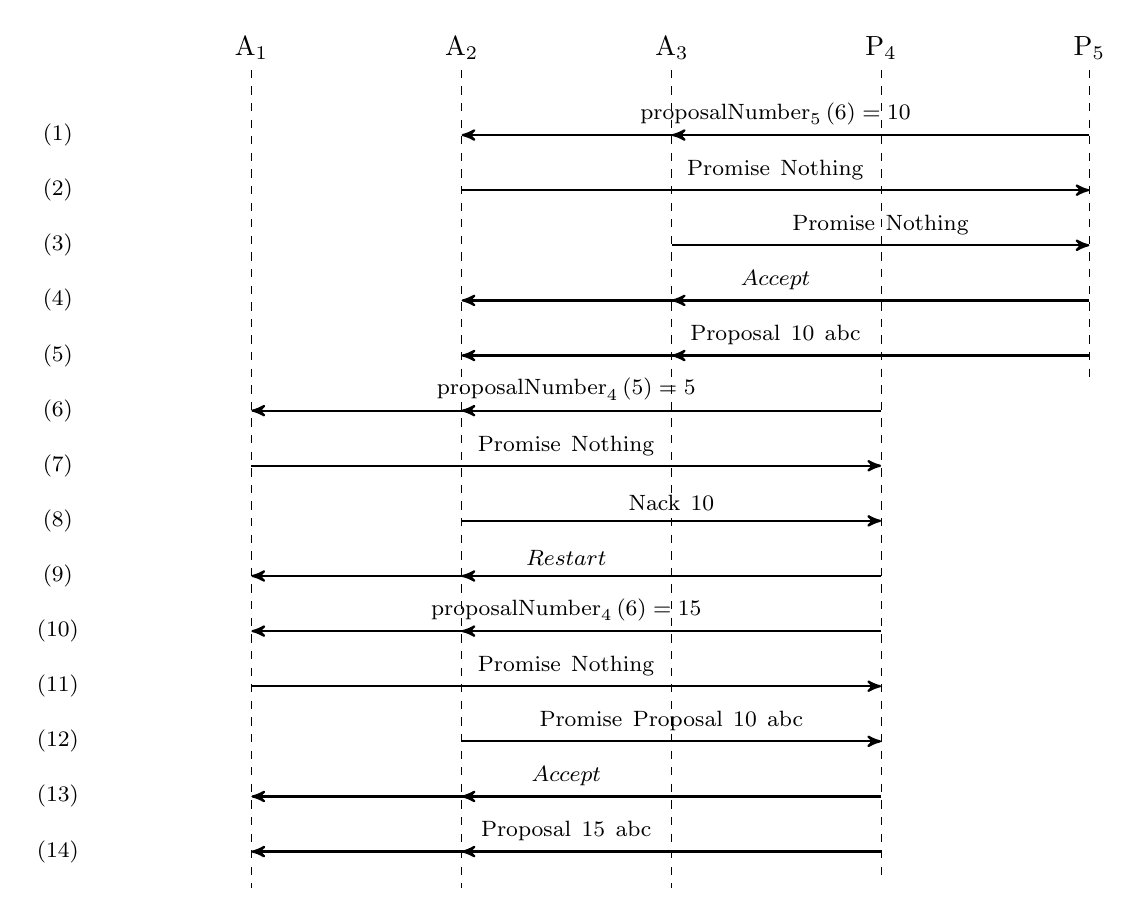
\begin{tikzpicture}[node distance=2cm, >=stealth', arrt/.style={above, font=\footnotesize}, arr/.style={->, thick}]
    \def\InitialOffset{0.4}
    \def\StepSize{0.7}
    \newcommand{\Step}[1]{\InitialOffset + #1 * \StepSize}
    \def\MaxSteps{14}
    \def\FullHeight{\Step{\MaxSteps} + 0.66 * \StepSize}

    \node (a1) {$\Acceptor{1}$};
    \node[right = of a1] (a2) {$\Acceptor{2}$};
    \node[right = of a2] (a3) {$\Acceptor{3}$};
    \node[right = of a3] (p4) {$\Proposer{4}$};
    \node[right = of p4] (p5) {$\Proposer{5}$};
    \node[left = of a1] (notes) {};

    \draw[dashed] (a1) -- ($(a1) - (0, \FullHeight)$);
    \draw[dashed] (a2) -- ($(a2) - (0, \FullHeight)$);
    \draw[dashed] (a3) -- ($(a3) - (0, \FullHeight)$);
    \draw[dashed] (p4) -- ($(p4) - (0, \Step{14.5})$);
    \draw[dashed] (p5) -- ($(p5) - (0, \Step{5.5})$);
    
    \draw[arr] ($(p5) - (0, \Step{1})$) -- node[arrt] {$\proposalNumber{6}{5} = 10$} ($(a2) - (0, \Step{1})$);
    \draw[arr] ($(p5) - (0, \Step{1})$) -- ($(a3) - (0, \Step{1})$);

    \draw[arr] ($(a2) - (0, \Step{2})$) -- node[arrt] {$\Promise{\Nothing}$} ($(p5) - (0, \Step{2})$);

    \draw[arr] ($(a3) - (0, \Step{3})$) -- node[arrt] {$\Promise{\Nothing}$} ($(p5) - (0, \Step{3})$);

    \draw[arr] ($(p5) - (0, \Step{4})$) -- node[arrt] {$\Accept$} ($(a2) - (0, \Step{4})$);
    \draw[arr] ($(p5) - (0, \Step{4})$) -- ($(a3) - (0, \Step{4})$);

    \draw[arr] ($(p5) - (0, \Step{5})$) -- node[arrt] {$\ProposalC{10}{\ABC}$} ($(a2) - (0, \Step{5})$);
    \draw[arr] ($(p5) - (0, \Step{5})$) -- ($(a3) - (0, \Step{5})$);

    \draw[arr] ($(p4) - (0, \Step{6})$) -- node[arrt] {$\proposalNumber{5}{4} = 5$} ($(a1) - (0, \Step{6})$);
    \draw[arr] ($(p4) - (0, \Step{6})$) -- ($(a2) - (0, \Step{6})$);

    \draw[arr] ($(a1) - (0, \Step{7})$) -- node[arrt] {$\Promise{\Nothing}$} ($(p4) - (0, \Step{7})$);

    \draw[arr] ($(a2) - (0, \Step{8})$) -- node[arrt] {$\Nack{10}$} ($(p4) - (0, \Step{8})$);

    \draw[arr] ($(p4) - (0, \Step{9})$) -- node[arrt] {$\Restart$} ($(a1) - (0, \Step{9})$);
    \draw[arr] ($(p4) - (0, \Step{9})$) -- ($(a2) - (0, \Step{9})$);

    \draw[arr] ($(p4) - (0, \Step{10})$) -- node[arrt] {$\proposalNumber{6}{4} = 15$} ($(a1) - (0, \Step{10})$);
    \draw[arr] ($(p4) - (0, \Step{10})$) -- ($(a2) - (0, \Step{10})$);

    \draw[arr] ($(a1) - (0, \Step{11})$) -- node[arrt] {$\Promise{\Nothing}$} ($(p4) - (0, \Step{11})$);
    
    \draw[arr] ($(a2) - (0, \Step{12})$) -- node[arrt] {$\Promise{\ProposalC{10}{\ABC}}$} ($(p4) - (0, \Step{12})$);

    \draw[arr] ($(p4) - (0, \Step{13})$) -- node[arrt] {$\Accept$} ($(a1) - (0, \Step{13})$);
    \draw[arr] ($(p4) - (0, \Step{13})$) -- ($(a2) - (0, \Step{13})$);

    \draw[arr] ($(p4) - (0, \Step{14})$) -- node[arrt] {$\ProposalC{15}{\ABC}$} ($(a1) - (0, \Step{14})$);
    \draw[arr] ($(p4) - (0, \Step{14})$) -- ($(a2) - (0, \Step{14})$);

    \foreach \r in {1,...,\MaxSteps} {
        \node[font=\footnotesize] at ($(notes) - (0, \Step{\r})$) {$(\r)$};
    }
\end{tikzpicture}
\caption{Example scenario with $3$ acceptors and $2$ proposers.}
\label{fig:scenario}
\end{figure}

\subsection{Scenario}
Figure \ref{fig:scenario} provides an overview where $\Acceptor{1}$, $\Acceptor{2}$, and $\Acceptor{3}$ are the acceptors and $\Proposer{4}$ and $\Proposer{5}$ are the proposers.
In steps $\Paren{1}$ to $\Paren{5}$, $\Proposer{5}$ completes the Paxos algorithm with $\Acceptor{2}$ and $\Acceptor{3}$ and terminates.

At this point $\Acceptor{2}$ has promised not to accept any proposal numbered less than $10$ and has accepted the value $\ABC$.
So, when $\Proposer{4}$ tries to use $4$ as its proposal number $\Paren{6}$, it receives $\Nack{10}$ from $\Acceptor{2}$ $\Paren{8}$ and has to restart the algorithm $\Paren{9}$.

$\Proposer{4}$ then runs through the Paxos algorithm with $\Acceptor{1}$ and $\Acceptor{2}$ starting with a new prepare request $\Paren{10}$ with a higher proposal number.
In step $\Paren{12}$ $\Proposer{4}$ learns that value $\ABC$ with proposal number $10$ has already been accepted by $\Acceptor{2}$.
Later, in step $\Paren{14}$, $\Proposer{4}$ issues a proposal with the value of the highest-numbered proposal that it receives as a response to its prepare request.
In this case there is only one such proposal, which is $\ProposalC{10}{\ABC}$.

In the end all $3$ acceptors have accepted the value $\ABC$.
$\Acceptor{1}$ and $\Acceptor{2}$ have accepted $\ProposalC{15}{\ABC}$ and $\Acceptor{3}$ has accepted $\ProposalC{10}{\ABC}$.

\subsection{Formulae}
We set $ac = 3$, $pc = 2$, and $V=\Curly{\ABC, \operatorname{def}, \dots, \operatorname{vwx}, \operatorname{yz}}$.

\subsubsection{System Initialization}
After inserting $ac$ and $pc$ and applying $\Init$ once we have:

$\Sys{ac}{pc} = \Sys{3}{2} =
\SessionAccept{a}{1}{t}.\ParallelFor{3 < i < 5} \PpInit{4}{\genAq{i}{3}{2}}{i}{i}{[]}\\
\Or \SessionRequest{a}{2}{t}.\PpInit{4}{\genAq{5}{3}{2}}{5}{5}{[]}\\
\Or \ParallelFor{1 \le j \le 3} \PaInit{j}{4}{3}{2}{n_j}{pr_j}$

% $\mapstostar \Init\\
% \Nu{t}\big (
% \PpInit{4}{A_{Q,1}}{4}{4}{[]} \Or \PpInit{4}{A_{Q,2}}{5}{5}{[]}\\
% \Or \PaInit{1}{4}{3}{2}{n_1}{pr_1} \Or \PaInit{2}{4}{3}{2}{n_2}{pr_2} \Or \PaInit{3}{4}{3}{2}{n_3}{pr_3}\\
% \Or \OuterSessionQueues
% \big )$

% $=\\
% % Is this step really necessary?
% \Nu{t}\big (
% \SessionRequest{b_4}{4}{s}.\Pp \Or \SessionRequest{b_5}{4}{r}.\Pp\\
% \Or \ParallelFor{3 < n \le 5} \SessionAccept{b_n}{1}{s} . \Pa\\
% \Or \ParallelFor{3 < n \le 5} \SessionAccept{b_n}{2}{s} . \Pa\\
% \Or \ParallelFor{3 < n \le 5} \SessionAccept{b_n}{3}{s} . \Pa\\
% \Or \OuterSessionQueues
% \big )$

$\mapstostar
\Nu{t}\big (
\SessionRequest{b_4}{4}{s}.\Pp \comment{= \Proposer{4}}\\
\Or \SessionRequest{b_5}{4}{r}.\Pp \comment{= \Proposer{5}}\\
\Or \Paren{\SessionAccept{b_4}{1}{s}.\Pa \Or \SessionAccept{b_5}{1}{r}.\Pa} \comment{= \Acceptor{1}}\\
\Or \Paren{\SessionAccept{b_4}{2}{s}.\Pa \Or \SessionAccept{b_5}{2}{r}.\Pa} \comment{= \Acceptor{2}}\\
\Or \Paren{\SessionAccept{b_4}{3}{s}.\Pa \Or \SessionAccept{b_5}{3}{r}.\Pa} \comment{= \Acceptor{3}}\\
\Or \OuterSessionQueues
\big )$

We apply $\Init$ thrice for shared-point $b_4$ and thrice again for shared-point $b_5$ to obtain:

$\mapstostar
\NuChannels\big (\\
\Mu{X} \update{n}{5} . \Paren{\DotForall{j\in \{1,2\}} \SendUnreliableP{s}{4}{j}{l1a}{\proposalNumber{n}{4}}}\dots \comment{= \Proposer{4}}\\
\Or \Mu{X} \update{n}{6} . \Paren{\DotForall{j\in \{2,3\}} \SendUnreliableP{r}{4}{j}{l1a}{\proposalNumber{n}{5}}}\dots \comment{= \Proposer{5}}\\
\Or \Paren{
    \Mu{X} \ReceiveUnreliableP{s}{4}{1}{l1a}{\perp}{n'}.\If{\dots}
    \Or \Mu{X} \ReceiveUnreliableP{r}{4}{1}{l1a}{\perp}{n'}.\If{\dots}
} \comment{= \Acceptor{1}}\\
\Or \Paren{
    \Mu{X} \ReceiveUnreliableP{s}{4}{2}{l1a}{\perp}{n'}.\If{\dots}
    \Or \Mu{X} \ReceiveUnreliableP{r}{4}{2}{l1a}{\perp}{n'}.\If{\dots}
} \comment{= \Acceptor{2}}\\
\Or \Paren{
    \Mu{X} \ReceiveUnreliableP{s}{4}{3}{l1a}{\perp}{n'}.\If{\dots}
    \Or \Mu{X} \ReceiveUnreliableP{r}{4}{3}{l1a}{\perp}{n'}.\If{\dots}
} \comment{= \Acceptor{3}}\\
\Or \InnerSessionQueues{s}
\Or \InnerSessionQueues{r}
\Or \OuterSessionQueues
\big )$

% $=\\
% \NuChannels\big (
% \Mu{X} \SendUnreliableP{s}{4}{1}{l1a}{\proposalNumber{5}{4}}.\SendUnreliableP{s}{4}{2}{l1a}{\proposalNumber{5}{4}}\dots\\
% \Or \Mu{X} \SendUnreliableP{r}{4}{2}{l1a}{\proposalNumber{6}{5}}.\SendUnreliableP{r}{4}{3}{l1a}{\proposalNumber{6}{5}}\dots\\
% \Or \Paren{
%     \Mu{X} \ReceiveUnreliableP{s}{4}{1}{l1a}{\perp}{n'}.\If{\dots}
%     \Or \Mu{X} \ReceiveUnreliableP{r}{4}{1}{l1a}{\perp}{n'}.\If{\dots}
% }\\
% \Or \Paren{
%     \Mu{X} \ReceiveUnreliableP{s}{4}{2}{l1a}{\perp}{n'}.\If{\dots}
%     \Or \Mu{X} \ReceiveUnreliableP{r}{4}{2}{l1a}{\perp}{n'}.\If{\dots}
% }\\
% \Or \Paren{
%     \Mu{X} \ReceiveUnreliableP{s}{4}{3}{l1a}{\perp}{n'}.\If{\dots}
%     \Or \Mu{X} \ReceiveUnreliableP{r}{4}{3}{l1a}{\perp}{n'}.\If{\dots}
% }\\
% \Or \InnerSessionQueues{s}
% \Or \InnerSessionQueues{r}
% \Or \OuterSessionQueues
% \big )$

Note that each process is shortened to only show the next few steps instead of the entire process.

\subsubsection{The Happy Path}
After applying the updates in $\Proposer{4}$ and $\Proposer{5}$ the first inter-process communication can take place.
In this case $\Proposer{5}$ communicates with $\Acceptor{2}$ and $\Acceptor{3}$.
We apply $\Usend$ and $\Uget$ twice to send $\proposalNumber{6}{5} = 10$ to $\Acceptor{2}$ and $\Acceptor{3}$.
% corresponds to (1)

$\mapstostar
\NuChannels \big (\\
\Mu{X} \SendUnreliableP{s}{4}{1}{l1a}{\proposalNumber{5}{4}}.\SendUnreliableP{s}{4}{2}{l1a}{\proposalNumber{5}{4}}\dots \comment{= \Proposer{4}}\\
\Or \Mu{X} \ReceiveUnreliableP{r}{2}{4}{l1b}{\perp}{v_2}.\ReceiveUnreliableP{r}{3}{4}{l1b}{\perp}{v_3}\dots \comment{= \Proposer{5}}\\
\Or \Paren{
    \Mu{X} \ReceiveUnreliableP{s}{4}{1}{l1a}{\perp}{n'}.\If{\dots}
    \Or \Mu{X} \ReceiveUnreliableP{r}{4}{1}{l1a}{\perp}{n'}.\If{\dots}
} \comment{=\Acceptor{1}}\\
\Or \Paren{
    \Mu{X} \ReceiveUnreliableP{s}{4}{2}{l1a}{\perp}{n'}.\If{\dots}
    \Or \Mu{X} \If{10 = \perp} \Then{\PaCont} \Else{\dots}
} \comment{=\Acceptor{2}}\\
\Or \Paren{
    \Mu{X} \ReceiveUnreliableP{s}{4}{3}{l1a}{\perp}{n'}.\If{\dots}
    \Or \Mu{X} \If{10 = \perp} \Then{\PaCont} \Else{\dots}
} \comment{=\Acceptor{3}}\\
\Or \InnerSessionQueues{s}
\Or \InnerSessionQueues{r}
\Or \OuterSessionQueues
\big )$

Since $10 \neq \perp$ both $\Acceptor{2}$ and $\Acceptor{3}$ move into their respective $\Else$ branches.

$=
\NuChannels \big (\\
\Mu{X} \SendUnreliableP{s}{4}{1}{l1a}{\proposalNumber{5}{4}}.\SendUnreliableP{s}{4}{2}{l1a}{\proposalNumber{5}{4}}\dots \comment{= \Proposer{4}}\\
\Or \Mu{X} \ReceiveUnreliableP{r}{2}{4}{l1b}{\perp}{v_2}.\ReceiveUnreliableP{r}{3}{4}{l1b}{\perp}{v_3}\dots \comment{= \Proposer{5}}\\
\Or \Paren{
    \Mu{X} \ReceiveUnreliableP{s}{4}{1}{l1a}{\perp}{n'}.\If{\dots}
    \Or \Mu{X} \ReceiveUnreliableP{r}{4}{1}{l1a}{\perp}{n'}.\If{\dots}
} \comment{=\Acceptor{1}}\\
\Or \Paren{
    \Mu{X} \ReceiveUnreliableP{s}{4}{2}{l1a}{\perp}{n'}.\If{\dots}
    \Or \Mu{X} \If{\greaterThan{10}{\Nothing}} \Then{\dots} \Else{\dots}
} \comment{=\Acceptor{2}}\\
\Or \Paren{
    \Mu{X} \ReceiveUnreliableP{s}{4}{3}{l1a}{\perp}{n'}.\If{\dots}
    \Or \Mu{X} \If{\greaterThan{10}{\Nothing}} \Then{\dots} \Else{\dots}
} \comment{=\Acceptor{3}}\\
\Or \InnerSessionQueues{s}
\Or \InnerSessionQueues{r}
\Or \OuterSessionQueues
\big )$

% % A1: n=Nothing, pr=Nothing
% % A2: n=10, pr=Nothing
% % A3: n=Nothing, pr=Nothing
% $=\\
% \NuChannels \big (
% \Mu{X} \SendUnreliableP{s}{4}{1}{l1a}{\proposalNumber{5}{4}}.\SendUnreliableP{s}{4}{2}{l1a}{\proposalNumber{5}{4}}\dots\\
% \Or \Mu{X} \SendUnreliableP{r}{4}{3}{l1a}{\proposalNumber{6}{5}}.\ReceiveUnreliableP{r}{2}{4}{l1b}{\perp}{v_2}\dots\\
% \Or \Paren{
%     \Mu{X} \ReceiveUnreliableP{s}{4}{1}{l1a}{\perp}{n'}.\If{\dots}
%     \Or \Mu{X} \ReceiveUnreliableP{r}{4}{1}{l1a}{\perp}{n'}.\If{\dots}
% }\\
% \Or \Paren{
%     \Mu{X} \ReceiveUnreliableP{s}{4}{2}{l1a}{\perp}{n'}.\If{\dots}
%     \Or \Mu{X} \SendUnreliableP{r}{2}{4}{l1b}{\Promise{\Nothing}}.\PaCont
% }\\
% \Or \Paren{
%     \Mu{X} \ReceiveUnreliableP{s}{4}{3}{l1a}{\perp}{n'}.\If{\dots}
%     \Or \Mu{X} \ReceiveUnreliableP{r}{4}{3}{l1a}{\perp}{n'}.\If{\dots}
% }\\
% \Or \InnerSessionQueues{s}
% \Or \InnerSessionQueues{r}
% \Or \OuterSessionQueues
% \big )$

Because $\greaterThan{10}{\Nothing}$ returns $\True$, $\Acceptor{2}$ and $\Acceptor{3}$ move into their respective $\Then$ branches.
After executing $\update{n}{10}$, $\Acceptor{2}$ and $\Acceptor{3}$ are ready to send their responses to $\Proposer{5}$.

% A1: n=Nothing, pr=Nothing
% A2: n=10, pr=Nothing
% A3: n=10, pr=Nothing
$=
\NuChannels \big (\\
\Mu{X} \SendUnreliableP{s}{4}{1}{l1a}{\proposalNumber{5}{4}}.\SendUnreliableP{s}{4}{2}{l1a}{\proposalNumber{5}{4}}\dots \comment{= \Proposer{4}}\\
\Or \Mu{X} \ReceiveUnreliableP{r}{2}{4}{l1b}{\perp}{v_2}.\ReceiveUnreliableP{r}{3}{4}{l1b}{\perp}{v_3}\dots \comment{= \Proposer{5}}\\
\Or \Paren{
    \Mu{X} \ReceiveUnreliableP{s}{4}{1}{l1a}{\perp}{n'}.\If{\dots}
    \Or \Mu{X} \ReceiveUnreliableP{r}{4}{1}{l1a}{\perp}{n'}.\If{\dots}
} \comment{= \Acceptor{1}}\\
\Or \Paren{
    \Mu{X} \ReceiveUnreliableP{s}{4}{2}{l1a}{\perp}{n'}.\If{\dots}
    \Or \Mu{X} \SendUnreliableP{r}{2}{4}{l1b}{\Promise{\Nothing}}.\PaCont
} \comment{= \Acceptor{2}}\\
\Or \Paren{
    \Mu{X} \ReceiveUnreliableP{s}{4}{3}{l1a}{\perp}{n'}.\If{\dots}
    \Or \Mu{X} \SendUnreliableP{r}{3}{4}{l1b}{\Promise{\Nothing}}.\PaCont
} \comment{= \Acceptor{3}}\\
\Or \InnerSessionQueues{s}
\Or \InnerSessionQueues{r}
\Or \OuterSessionQueues
\big )$

We apply $\Usend$ and $\Uget$ twice to do just that.
Note that we also apply $\Uskip$ to $\Acceptor{1}$ and evaluate its branches.
All three acceptors move into $\PaCont$.
% corresponds to (2) - (3)

% $\mapstostar (USkip)\\
% \NuChannels \big (
% \Mu{X} \SendUnreliableP{s}{4}{1}{l1a}{\proposalNumber{5}{4}}.\SendUnreliableP{s}{4}{2}{l1a}{\proposalNumber{5}{4}}\dots\\
% \Or \Mu{X} \ReceiveUnreliableP{r}{2}{4}{l1b}{\perp}{v_2}.\ReceiveUnreliableP{r}{3}{4}{l1b}{\perp}{v_3}\dots\\
% \Or \Paren{
%     \Mu{X} \ReceiveUnreliableP{s}{4}{1}{l1a}{\perp}{n'}.\If{\dots}
%     \Or \Mu{X} \If{\perp = \perp} \Then{\PaCont} \Else{\dots}
% }\\
% \Or \Paren{
%     \Mu{X} \ReceiveUnreliableP{s}{4}{2}{l1a}{\perp}{n'}.\If{\dots}
%     \Or \Mu{X} \SendUnreliableP{r}{2}{4}{l1b}{\Promise{\Nothing}}.\PaCont
% }\\
% \Or \Paren{
%     \Mu{X} \ReceiveUnreliableP{s}{4}{3}{l1a}{\perp}{n'}.\If{\dots}
%     \Or \Mu{X} \SendUnreliableP{r}{3}{4}{l1b}{\Promise{\Nothing}}.\PaCont
% }\\
% \Or \InnerSessionQueues{s}
% \Or \InnerSessionQueues{r}
% \Or \OuterSessionQueues
% \big )$

% $=\\
% \NuChannels \big (
% \Mu{X} \SendUnreliableP{s}{4}{1}{l1a}{\proposalNumber{5}{4}}.\SendUnreliableP{s}{4}{2}{l1a}{\proposalNumber{5}{4}}\dots\\
% \Or \Mu{X} \ReceiveUnreliableP{r}{2}{4}{l1b}{\perp}{v_2}.\ReceiveUnreliableP{r}{3}{4}{l1b}{\perp}{v_3}\dots\\
% \Or \Paren{
%     \Mu{X} \ReceiveUnreliableP{s}{4}{1}{l1a}{\perp}{n'}.\If{\dots}
%     \Or \Mu{X} \ReceiveWeaklyP{r}{4}{1}{\Accept \dots \oplus \Restart .X \oplus \Abort .end}
% }\\
% \Or \Paren{
%     \Mu{X} \ReceiveUnreliableP{s}{4}{2}{l1a}{\perp}{n'}.\If{\dots}
%     \Or \Mu{X} \SendUnreliableP{r}{2}{4}{l1b}{\Promise{\Nothing}}.\PaCont
% }\\
% \Or \Paren{
%     \Mu{X} \ReceiveUnreliableP{s}{4}{3}{l1a}{\perp}{n'}.\If{\dots}
%     \Or \Mu{X} \SendUnreliableP{r}{3}{4}{l1b}{\Promise{\Nothing}}.\PaCont
% }\\
% \Or \InnerSessionQueues{s}
% \Or \InnerSessionQueues{r}
% \Or \OuterSessionQueues
% \big )$

% $\mapstostar (USend + UGet)\\
% \NuChannels \big (
% \Mu{X} \SendUnreliableP{s}{4}{1}{l1a}{\proposalNumber{5}{4}}.\SendUnreliableP{s}{4}{2}{l1a}{\proposalNumber{5}{4}}\dots\\
% \Or \Mu{X} \ReceiveUnreliableP{r}{3}{4}{l1b}{\perp}{v_3}.\If{\anyNack{\VectorV} \tOr \promiseCount{\VectorV} < 1} \Then{\dots}\\
% \Or \Paren{
%     \Mu{X} \ReceiveUnreliableP{s}{4}{1}{l1a}{\perp}{n'}.\If{\dots}
%     \Or \Mu{X} \ReceiveWeaklyP{r}{4}{1}{\BeginPaCont}
% }\\
% \Or \Paren{
%     \Mu{X} \ReceiveUnreliableP{s}{4}{2}{l1a}{\perp}{n'}.\If{\dots}
%     \Or \Mu{X} \ReceiveWeaklyP{r}{4}{2}{\BeginPaCont}
% }\\
% \Or \Paren{
%     \Mu{X} \ReceiveUnreliableP{s}{4}{3}{l1a}{\perp}{n'}.\If{\dots}
%     \Or \Mu{X} \SendUnreliableP{r}{3}{4}{l1b}{\Promise{\Nothing}}.\PaCont
% }\\
% \Or \InnerSessionQueues{s}
% \Or \InnerSessionQueues{r}
% \Or \OuterSessionQueues
% \big )$

% $\mapstostar (USend + UGet)\\
% \NuChannels \big (
% \Mu{X} \SendUnreliableP{s}{4}{1}{l1a}{\proposalNumber{5}{4}}.\SendUnreliableP{s}{4}{2}{l1a}{\proposalNumber{5}{4}}\dots\\
% \Or \Mu{X} \If{\False \tOr 2 < 1} \Then{\dots} \Else{\SendWeaklyP{r}{4}{\Curly{2,3}}{\Accept}{\dots}}\\
% \Or \Paren{
%     \Mu{X} \ReceiveUnreliableP{s}{4}{1}{l1a}{\perp}{n'}.\If{\dots}
%     \Or \Mu{X} \ReceiveWeaklyP{r}{4}{1}{\BeginPaCont}
% }\\
% \Or \Paren{
%     \Mu{X} \ReceiveUnreliableP{s}{4}{2}{l1a}{\perp}{n'}.\If{\dots}
%     \Or \Mu{X} \ReceiveWeaklyP{r}{4}{2}{\BeginPaCont}
% }\\
% \Or \Paren{
%     \Mu{X} \ReceiveUnreliableP{s}{4}{3}{l1a}{\perp}{n'}.\If{\dots}
%     \Or \Mu{X} \ReceiveWeaklyP{r}{4}{3}{\BeginPaCont}
% }\\
% \Or \InnerSessionQueues{s}
% \Or \InnerSessionQueues{r}
% \Or \OuterSessionQueues
% \big )$

$\mapstostar
\NuChannels \big (\\
\Mu{X} \SendUnreliableP{s}{4}{1}{l1a}{\proposalNumber{5}{4}}.\SendUnreliableP{s}{4}{2}{l1a}{\proposalNumber{5}{4}}\dots \comment{= \Proposer{4}}\\
\Or \Mu{X} \SendWeaklyP{r}{4}{\Curly{2,3}}{\Accept}{\SendUnreliableP{r}{4}{2}{l2a}{\ProposalC{10}{\ABC}}}\dots \comment{= \Proposer{5}}\\
\Or \Paren{
    \Mu{X} \dots
    \Or \Mu{X} \ReceiveWeaklyP{r}{4}{1}{\BeginPaCont}
} \comment{= \Acceptor{1}}\\
\Or \Paren{
    \Mu{X} \dots
    \Or \Mu{X} \ReceiveWeaklyP{r}{4}{2}{\BeginPaCont}
} \comment{= \Acceptor{2}}\\
\Or \Paren{
    \Mu{X} \dots
    \Or \Mu{X} \ReceiveWeaklyP{r}{4}{3}{\BeginPaCont}
} \comment{= \Acceptor{3}}\\
\Or \InnerSessionQueues{s}
\Or \InnerSessionQueues{r}
\Or \OuterSessionQueues
\big )$

$\Proposer{5}$ broadcasts its decision $\Accept$ to $\Acceptor{2}$ and $\Acceptor{3}$.
By applying $\Wsel$ once, $\Wbran$ twice we obtain:
% corresponds to (4)

$\mapstostar
\NuChannels \big (\\
\Mu{X} \SendUnreliableP{s}{4}{1}{l1a}{\proposalNumber{5}{4}}.\SendUnreliableP{s}{4}{2}{l1a}{\proposalNumber{5}{4}}\dots \comment{= \Proposer{4}}\\
\Or \Mu{X} \SendUnreliableP{r}{4}{2}{l2a}{\ProposalC{10}{\ABC}}.\SendUnreliableP{r}{4}{3}{l2a}{\ProposalC{10}{\ABC}}\dots \comment{= \Proposer{5}}\\
\Or \Paren{
    \Mu{X} \dots
    \Or \Mu{X} \ReceiveWeaklyP{r}{4}{1}{\BeginPaCont}
} \comment{= \Acceptor{1}}\\
\Or \Paren{
    \Mu{X} \dots
    \Or \Mu{X} \ReceiveUnreliableP{r}{4}{2}{l2a}{\perp}{pr'}.\If{\dots}
} \comment{= \Acceptor{2}}\\
\Or \Paren{
    \Mu{X} \dots
    \Or \Mu{X} \ReceiveUnreliableP{r}{4}{3}{l2a}{\perp}{pr'}.\If{\dots}
} \comment{= \Acceptor{3}}\\
\Or \InnerSessionQueues{s}
\Or \InnerSessionQueues{r}
\Or \OuterSessionQueues
\big )$

% $\mapstostar (WSkip)\\
% \NuChannels \big (
% \Mu{X} \SendUnreliableP{s}{4}{1}{l1a}{\proposalNumber{5}{4}}.\SendUnreliableP{s}{4}{2}{l1a}{\proposalNumber{5}{4}}\dots\\
% \Or \Mu{X} \SendUnreliableP{r}{4}{2}{l2a}{\ProposalC{\proposalNumber{5}{6}}{\promValue{\VectorV}}}.\\\hspace*{1em}\SendUnreliableP{r}{4}{3}{l2a}{\ProposalC{\proposalNumber{5}{6}}{\promValue{\VectorV}}}\dots\\
% \Or \Paren{
%     \Mu{X} \ReceiveUnreliableP{s}{4}{1}{l1a}{\perp}{n'}.\If{\dots}
%     \Or \Mu{X} end
% }\\
% \Or \Paren{
%     \Mu{X} \ReceiveUnreliableP{s}{4}{2}{l1a}{\perp}{n'}.\If{\dots}
%     \Or \Mu{X} \ReceiveUnreliableP{r}{4}{2}{l2a}{\perp}{pr'}.\If{\dots}
% }\\
% \Or \Paren{
%     \Mu{X} \ReceiveUnreliableP{s}{4}{3}{l1a}{\perp}{n'}.\If{\dots}
%     \Or \Mu{X} \ReceiveUnreliableP{r}{4}{3}{l2a}{\perp}{pr'}.\If{\dots}
% }\\
% \Or \InnerSessionQueues{s}
% \Or \InnerSessionQueues{r}
% \Or \OuterSessionQueues
% \big )$

% $\mapstostar (USend + UGet)\\
% \NuChannels \big (
% \Mu{X} \SendUnreliableP{s}{4}{1}{l1a}{\proposalNumber{5}{4}}.\SendUnreliableP{s}{4}{2}{l1a}{\proposalNumber{5}{4}}\dots\\
% \Or \Mu{X} \SendUnreliableP{r}{4}{3}{l2a}{\ProposalC{\proposalNumber{5}{6}}{\promValue{\VectorV}}}.end\\
% \Or \Mu{X} \ReceiveUnreliableP{s}{4}{1}{l1a}{\perp}{n'}.\If{\dots}\\
% \Or \Paren{
%     \Mu{X} \ReceiveUnreliableP{s}{4}{2}{l1a}{\perp}{n'}.\If{\dots}
%     \Or \Mu{X} \If{\ProposalC{10}{\ABC} = \perp} \Then{X} \Else{\dots}
% }\\
% \Or \Paren{
%     \Mu{X} \ReceiveUnreliableP{s}{4}{3}{l1a}{\perp}{n'}.\If{\dots}
%     \Or \Mu{X} \ReceiveUnreliableP{r}{4}{3}{l2a}{\perp}{pr'}.\If{\dots}
% }\\
% \Or \InnerSessionQueues{s}
% \Or \InnerSessionQueues{r}
% \Or \OuterSessionQueues
% \big )$

% $\mapstostar (USend + UGet)\\
% \NuChannels \big (
% \Mu{X} \SendUnreliableP{s}{4}{1}{l1a}{\proposalNumber{5}{4}}.\SendUnreliableP{s}{4}{2}{l1a}{\proposalNumber{5}{4}}\dots\\
% \Or \Mu{X} end\\
% \Or \Mu{X} \ReceiveUnreliableP{s}{4}{1}{l1a}{\perp}{n'}.\If{\dots}\\
% \Or \Paren{
%     \Mu{X} \ReceiveUnreliableP{s}{4}{2}{l1a}{\perp}{n'}.\If{\dots}
%     \Or \Mu{X} \If{\ProposalC{10}{\ABC} = \perp} \Then{X} \Else{\dots}
% }\\
% \Or \Paren{
%     \Mu{X} \ReceiveUnreliableP{s}{4}{3}{l1a}{\perp}{n'}.\If{\dots}
%     \Or \Mu{X} \If{\ProposalC{10}{\ABC} = \perp} \Then{X} \Else{\dots}
% }\\
% \Or \InnerSessionQueues{s}
% \Or \InnerSessionQueues{r}
% \Or \OuterSessionQueues
% \big )$

% $=\\
% \NuChannels \big (
% \Mu{X} \SendUnreliableP{s}{4}{1}{l1a}{\proposalNumber{5}{4}}.\SendUnreliableP{s}{4}{2}{l1a}{\proposalNumber{5}{4}}\dots\\
% \Or \Mu{X} \ReceiveUnreliableP{s}{4}{1}{l1a}{\perp}{n'}.\If{\dots}\\
% \Or (
%     \Mu{X} \ReceiveUnreliableP{s}{4}{2}{l1a}{\perp}{n'}.\If{\dots}
%     \\\hspace*{1em}\Or \Mu{X} \If{\greaterEqual{10}{10}} \Then{\update{pr}{pr'}.\update{n}{\Just{10}}.X} \Else{\dots}
% )\\
% \Or (
%     \Mu{X} \ReceiveUnreliableP{s}{4}{3}{l1a}{\perp}{n'}.\If{\dots}
%     \\\hspace*{1em}\Or \Mu{X} \If{\greaterEqual{10}{10}} \Then{\update{pr}{pr'}.\update{n}{\Just{10}}.X} \Else{\dots}
% )\\
% \Or \InnerSessionQueues{s}
% \Or \InnerSessionQueues{r}
% \Or \OuterSessionQueues
% \big )$

% % A1: n=Nothing, pr=Nothing
% % A2: n=10, pr=Proposal 10 abc
% % A3: n=10, pr=Proposal 10 abc
% $=\\
% \NuChannels \big (
% \Mu{X} \SendUnreliableP{s}{4}{1}{l1a}{\proposalNumber{5}{4}}.\SendUnreliableP{s}{4}{2}{l1a}{\proposalNumber{5}{4}}\dots\\
% \Or \Mu{X} \ReceiveUnreliableP{s}{4}{1}{l1a}{\perp}{n'}.\If{\dots}\\
% \Or \Paren{
%     \Mu{X} \ReceiveUnreliableP{s}{4}{2}{l1a}{\perp}{n'}.\If{\dots}
%     \Or \Mu{X} X
% }\\
% \Or \Paren{
%     \Mu{X} \ReceiveUnreliableP{s}{4}{3}{l1a}{\perp}{n'}.\If{\dots}
%     \Or \Mu{X} X
% }\\
% \Or \InnerSessionQueues{s}
% \Or \InnerSessionQueues{r}
% \Or \OuterSessionQueues
% \big )$

Now $\Proposer{5}$ can send its proposal to $\Acceptor{2}$ and $\Acceptor{3}$ and terminate.
To do so we apply $\Usend$ and $\Uget$ twice.
$\Acceptor{2}$ and $\Acceptor{3}$ accept the proposal and the respective subprocesses terminate.
Note that we apply $\Wskip$ in $\Acceptor{1}$ and terminate that subprocess as well.
% corresponds to (5)

$\mapstostar
\NuChannels \big (\\
\Mu{X} \SendUnreliableP{s}{4}{1}{l1a}{\proposalNumber{5}{4}}.\SendUnreliableP{s}{4}{2}{l1a}{\proposalNumber{5}{4}}\dots \comment{= \Proposer{4}}\\
\Or \Mu{X} \ReceiveUnreliableP{s}{4}{1}{l1a}{\perp}{n'}.\If{\dots} \comment{= \Acceptor{1}}\\
\Or \Mu{X} \ReceiveUnreliableP{s}{4}{2}{l1a}{\perp}{n'}.\If{\dots} \comment{= \Acceptor{2}}\\
\Or \Mu{X} \ReceiveUnreliableP{s}{4}{3}{l1a}{\perp}{n'}.\If{\dots} \comment{= \Acceptor{3}}\\
\Or \InnerSessionQueues{s}
\Or \InnerSessionQueues{r}
\Or \OuterSessionQueues
\big )$

At this point the local variables of $\Acceptor{2}$ and $\Acceptor{3}$ are $n = 10$ and $pr = \ProposalC{10}{\ABC}$.
$\Acceptor{1}$ has not updated its local variables $n = \Nothing$ and $pr = \Nothing$.

\subsubsection{Restarting the Algorithm}
Next, $\Proposer{4}$ sends prepare requests with a proposal number less than 10, which is rejected by $\Acceptor{2}$.
$\Proposer{4}$ then decides to restart the algorithm.
We apply $\Usend$ and $\Uget$ twice.
We also apply $\Uskip$ once in $\Acceptor{3}$.

$\mapstostar
\NuChannels \big (\\
\Mu{X} \ReceiveUnreliableP{s}{1}{4}{l1b}{\perp}{v_1}.\ReceiveUnreliableP{s}{2}{4}{l1b}{\perp}{v_2}\dots \comment{= \Proposer{4}}\\
\Or \Mu{X} \If{5 = \perp} \Then{\PaCont} \Else{\dots} \comment{= \Acceptor{1}}\\
\Or \Mu{X} \If{5 = \perp} \Then{\PaCont} \Else{\dots} \comment{= \Acceptor{2}}\\
\Or \Mu{X} \If{\perp = \perp} \Then{\PaCont} \Else{\dots} \comment{= \Acceptor{3}}\\
\Or \InnerSessionQueues{s}
\Or \InnerSessionQueues{r}
\Or \OuterSessionQueues
\big )$

$\Acceptor{3}$ moves directly to $\PaCont$ whereas $\Acceptor{1}$ and $\Acceptor{2}$ send their responses to $\Proposer{4}$ before moving to $\PaCont$.
$\Acceptor{1}$ also updates its local variable $n = 5$.

% $=\\
% \NuChannels \big (
% \Mu{X} \ReceiveUnreliableP{s}{1}{4}{l1b}{\perp}{v_1}.\ReceiveUnreliableP{s}{2}{4}{l1b}{\perp}{v_2}\dots\\
% \Or \Mu{X} \If{\greaterThan{5}{\Nothing}} \Then{\update{n}{5}\dots}\Else{\dots}\\
% \Or \Paren{
%     \Mu{X} \If{\greaterThan{5}{\Just{10}}} \Then{\dots} \Else{\SendUnreliableP{s}{2}{4}{l1b}{\Nack{10}}.\PaCont}
%     \Or \Mu{X} X
% }\\
% \Or \Paren{
%     \Mu{X} \ReceiveWeaklyP{r}{4}{3}{\BeginPaCont}
%     \Or \Mu{X} X
% }\\
% \Or \InnerSessionQueues{s}
% \Or \InnerSessionQueues{r}
% \Or \OuterSessionQueues
% \big )$

% A1: n=5, pr=Nothing
% A2: n=10, pr=Proposal 10 abc
% A3: n=10, pr=Proposal 10 abc
$=
\NuChannels \big (\\
\Mu{X} \ReceiveUnreliableP{s}{1}{4}{l1b}{\perp}{v_1}.\ReceiveUnreliableP{s}{2}{4}{l1b}{\perp}{v_2}\dots \comment{= \Proposer{4}}\\
\Or \Mu{X} \SendUnreliableP{s}{1}{4}{l1b}{\Promise{\Nothing}}.\PaCont \comment{= \Acceptor{1}}\\
\Or \Mu{X} \SendUnreliableP{s}{2}{4}{l1b}{\Nack{10}}.\PaCont \comment{= \Acceptor{2}}\\
\Or \Mu{X} \ReceiveWeaklyP{r}{4}{3}{\BeginPaCont} \comment{= \Acceptor{3}}\\
\Or \InnerSessionQueues{s}
\Or \InnerSessionQueues{r}
\Or \OuterSessionQueues
\big )$

% $\mapstostar (USend + UGet, USend + UGet)\\
% \NuChannels \big (
% \Mu{X} \If{\True \tOr 1 < 1} \Then{\SendWeaklyP{s}{4}{\Curly{1,2}}{\Restart}{X}} \Else{\dots}\\
% \Or \Mu{X} \ReceiveWeaklyP{s}{4}{1}{\BeginPaCont}\\
% \Or \Paren{
%     \Mu{X} \ReceiveWeaklyP{s}{4}{1}{\BeginPaCont}
%     \Or \Mu{X} X
% }\\
% \Or \Paren{
%     \Mu{X} \ReceiveWeaklyP{r}{4}{3}{\BeginPaCont}
%     \Or \Mu{X} X
% }\\
% \Or \InnerSessionQueues{s}
% \Or \InnerSessionQueues{r}
% \Or \OuterSessionQueues
% \big )$

Applying $\Usend$ and $\Uget$ twice and evaluating the branching in $\Proposer{4}$ yields:

$\mapstostar
\NuChannels \big (\\
\Mu{X} \SendWeaklyP{s}{4}{\Curly{1,2}}{\Restart}{X}\\
\Or \Mu{X} \ReceiveWeaklyP{s}{4}{1}{\BeginPaCont}\\
\Or \Mu{X} \ReceiveWeaklyP{s}{4}{1}{\BeginPaCont}\\
\Or \Mu{X} \ReceiveWeaklyP{r}{4}{3}{\BeginPaCont}\\
\Or \InnerSessionQueues{s}
\Or \InnerSessionQueues{r}
\Or \OuterSessionQueues
\big )$

% $\mapstostar (WSel + WBran, WSkip)\\
% \NuChannels \big (
% \Mu{X} X\\
% \Or \Mu{X} X\\
% \Or \Paren{
%     \Mu{X} X
%     \Or \Mu{X} X
% }\\
% \Or \Paren{
%     \Mu{X} end
%     \Or \Mu{X} X
% }\\
% \Or \InnerSessionQueues{s}
% \Or \InnerSessionQueues{r}
% \Or \OuterSessionQueues
% \big )$

$\Proposer{4}$ sends its decision to restart the algorithm to $\Acceptor{1}$ and $\Acceptor{2}$ by applying $\Wsel$ once and $\Wbran$ twice.
$\Acceptor{3}$ terminates after applying $\Wskip$.

$\mapstostar
\NuChannels \big (\\
\Mu{X} \SendUnreliableP{s}{4}{1}{l1a}{15}.\SendUnreliableP{s}{4}{2}{l1a}{15}\dots \comment{= \Proposer{4}}\\
\Or \Mu{X} \ReceiveUnreliableP{s}{4}{1}{l1a}{\perp}{n'}.\If{\dots} \comment{= \Acceptor{1}}\\
\Or \Mu{X} \ReceiveUnreliableP{s}{4}{2}{l1a}{\perp}{n'}.\If{\dots} \comment{= \Acceptor{2}}\\
\Or \InnerSessionQueues{s}
\Or \InnerSessionQueues{r}
\Or \OuterSessionQueues
\big )$

% $\mapstostar (USend + UGet, USend + UGet)\\
% \NuChannels \big (
% \Mu{X} \ReceiveUnreliableP{s}{1}{4}{l1b}{\perp}{v_1}.\ReceiveUnreliableP{s}{2}{4}{l1b}{\perp}{v_2}.\If{\dots}\\
% \Or \Mu{X} \If{15 = \perp} \Then{\PaCont} \Else{\dots}\\
% \Or \Paren{
%     \Mu{X} \If{15 = \perp} \Then{\PaCont} \Else{\dots}
%     \Or \Mu{X} X
% }\\
% \Or \Mu{X} X\\
% \Or \InnerSessionQueues{s}
% \Or \InnerSessionQueues{r}
% \Or \OuterSessionQueues
% \big )$

% % A1: n=5, pr=Nothing
% % A2: n=10, pr=Proposal 10 abc
% % A3: n=10, pr=Proposal 10 abc
% $\mapstostar
% \NuChannels \big (\\
% \Mu{X} \ReceiveUnreliableP{s}{1}{4}{l1b}{\perp}{v_1}.\ReceiveUnreliableP{s}{2}{4}{l1b}{\perp}{v_2}.\If{\dots}\\
% \Or \Mu{X} \If{\greaterThan{15}{\Just{5}}} \Then{\update{n}{15}\dots} \Else{\dots}\\
% \Or \Mu{X} \If{\greaterThan{15}{\Just{10}}} \Then{\update{n}{15}\dots} \Else{\dots}\\
% \Or \InnerSessionQueues{s}
% \Or \InnerSessionQueues{r}
% \Or \OuterSessionQueues
% \big )$

\subsubsection{The Happy Path, Again}

This time $\Proposer{4}$ uses a high enough proposal number so that $\Acceptor{1}$ and $\Acceptor{2}$ both promise not to accept any proposal numbered less than that.
By applying $\Usend$ and $\Uget$ and evaluating the branches in the remaining acceptors we arrive at:

% A1: n=15, pr=Nothing
% A2: n=15, pr=Proposal 10 abc
% A3: n=10, pr=Proposal 10 abc
$\mapstostar
\NuChannels \big (\\
\Mu{X} \ReceiveUnreliableP{s}{1}{4}{l1b}{\perp}{v_1}.\ReceiveUnreliableP{s}{2}{4}{l1b}{\perp}{v_2}.\If{\dots} \comment{= \Proposer{4}}\\
\Or \Mu{X} \SendUnreliableP{s}{1}{4}{l1b}{\Promise{\Nothing}}.\PaCont \comment{= \Acceptor{1}}\\
\Or \Mu{X} \SendUnreliableP{s}{2}{4}{l1b}{\Promise{\ProposalC{10}{abc}}}.\PaCont \comment{= \Acceptor{2}}\\
\Or \InnerSessionQueues{s}
\Or \InnerSessionQueues{r}
\Or \OuterSessionQueues
\big )$

Note that, at this point, $\Acceptor{1}$ and $\Acceptor{2}$ have updated their respective $n$ to $15$.

Because $\Acceptor{2}$ has already accepted a proposal, it responds to $\Proposer{4}$'s prepare request with that proposal.
Twice more we apply $\Usend$ and $\Uget$ and evaluate the branch in $\Proposer{4}$ to obtain:

% % A1: n=15, pr=Nothing
% % A2: n=15, pr=Proposal 10 abc
% % A3: n=10, pr=Proposal 10 abc
% $\mapstostar (USend + UGet, USend + UGet)\\
% \NuChannels \big (
% \Mu{X} \If{\False \tOr 2 < 1} \Then{\dots} \Else{\SendWeaklyP{s}{4}{\Curly{1,2}}{\Accept}{\dots}}\\
% \Or \Mu{X} \ReceiveWeaklyP{s}{4}{1}{\BeginPaCont}\\
% \Or \Paren{
%     \Mu{X} \ReceiveWeaklyP{s}{4}{1}{\BeginPaCont}
%     \Or \Mu{X} X
% }\\
% \Or \Mu{X} X\\
% \Or \InnerSessionQueues{s}
% \Or \InnerSessionQueues{r}
% \Or \OuterSessionQueues
% \big )$

% A1: n=15, pr=Nothing
% A2: n=15, pr=Proposal 10 abc
% A3: n=10, pr=Proposal 10 abc
$\mapstostar
\NuChannels \big (\\
\Mu{X} \SendWeaklyP{s}{4}{\Curly{1,2}}{\Accept}{\dots} \comment{= \Proposer{4}}\\
\Or \Mu{X} \ReceiveWeaklyP{s}{4}{1}{\BeginPaCont} \comment{= \Acceptor{1}}\\
\Or \Mu{X} \ReceiveWeaklyP{s}{4}{1}{\BeginPaCont} \comment{= \Acceptor{2}}\\
\Or \InnerSessionQueues{s}
\Or \InnerSessionQueues{r}
\Or \OuterSessionQueues
\big )$

$\Proposer{4}$ has received enough promises to send its own proposal.
The value for that proposal is $\ABC$ because that is the value of the highest-numbered proposal $\Proposer{4}$ received as a response to its prepare request.
First, we apply $\Wsel$ and $\Wbran$.

% A1: n=15, pr=Nothing
% A2: n=15, pr=Proposal 10 abc
% A3: n=10, pr=Proposal 10 abc
$\mapstostar
\NuChannels \big (\\
\Mu{X} \SendUnreliableP{s}{4}{1}{l2a}{\ProposalC{15}{\ABC}}.
\SendUnreliableP{s}{4}{2}{l2a}{\ProposalC{15}{\ABC}}.end \comment{= \Proposer{4}}\\
\Or \Mu{X} \ReceiveUnreliableP{s}{4}{1}{l2a}{\perp}{pr'}.\If{\dots}\comment{= \Acceptor{1}}\\
\Or \Mu{X} \ReceiveUnreliableP{s}{4}{2}{l2a}{\perp}{pr'}.\If{\dots}\comment{= \Acceptor{2}}\\
\Or \InnerSessionQueues{s}
\Or \InnerSessionQueues{r}
\Or \OuterSessionQueues
\big )$

Then we apply $\Usend$ and $\Uget$ to send the proposal from $\Proposer{4}$ to the acceptors.
$\Proposer{4}$ terminates and the acceptors accept the received proposal and then terminate as well.

% % A1: n=15, pr=Nothing
% % A2: n=15, pr=Proposal 10 abc
% % A3: n=10, pr=Proposal 10 abc
% $\mapstostar (USend + UGet, USend + UGet)\\
% \NuChannels \big (
% \Mu{X} end\\
% \Or \Mu{X} \If{\ProposalC{15}{\ProposalC{15}{abc}} = \perp} \Then{\dots} \Else{\dots}\\
% \Or \Paren{
%     \Mu{X} \If{\ProposalC{15}{\ProposalC{15}{abc}} = \perp} \Then{\dots} \Else{\dots}
%     \Or \Mu{X} X
% }\\
% \Or \Mu{X} X\\
% \Or \InnerSessionQueues{s}
% \Or \InnerSessionQueues{r}
% \Or \OuterSessionQueues
% \big )$

% % A1: n=15, pr=Nothing
% % A2: n=15, pr=Proposal 10 abc
% % A3: n=10, pr=Proposal 10 abc
% $=\\
% \NuChannels \big (
% \Or \Mu{X} \If{\greaterEqual{15}{\Just{15}}}\\\hspace*{1em}\Then{\update{pr}{\ProposalC{15}{abc}}.\update{n}{15}.X} \Else{\dots}\\
% \Or (
%     \Mu{X} \If{\greaterEqual{15}{\Just{15}}}\\\hspace*{1em}\Then{\update{pr}{\ProposalC{15}{abc}}.\update{n}{15}.X} \Else{\dots}
%     \Or \Mu{X} X
% )\\
% \Or \Mu{X} X\\
% \Or \InnerSessionQueues{s}
% \Or \InnerSessionQueues{r}
% \Or \OuterSessionQueues
% \big )$

% % A1: n=15, pr=Proposal 15 abc
% % A2: n=15, pr=Proposal 15 abc
% % A3: n=10, pr=Proposal 10 abc
% $=\\
% \NuChannels \big (
% \Or \Mu{X} X\\
% \Or \Paren{
%     \Mu{X} X
%     \Or \Mu{X} X
% }\\
% \Or \Mu{X} X\\
% \Or \InnerSessionQueues{s}
% \Or \InnerSessionQueues{r}
% \Or \OuterSessionQueues
% \big )$

% A1: n=15, pr=Proposal 15 abc
% A2: n=15, pr=Proposal 15 abc
% A3: n=10, pr=Proposal 10 abc
$\mapstostar
\NuChannels \big (\InnerSessionQueues{s}
\Or \InnerSessionQueues{r}
\Or \OuterSessionQueues
\big )$

Afterwards $\Acceptor{1}$ and $\Acceptor{2}$ have $n = 15$ and $pr = \ProposalC{15}{\ABC}$ and $\Acceptor{3}$ has $n = 10$ and $pr = \ProposalC{10}{\ABC}$.
All acceptors have accepted the value $\ABC$.

% % A1: n=15, pr=Proposal 15 abc
% % A2: n=15, pr=Proposal 15 abc
% % A3: n=10, pr=Proposal 10 abc
% $=\\
% \NuChannels \Paren{
%     \Or \InnerSessionQueues{s}
%     \Or \InnerSessionQueues{r}
%     \Or \OuterSessionQueues
% }$



\chapter{Analysis}
We take the model from the previous chapter, type-check it, and discuss what the type check means for agreement, validity, and termination of the Paxos algorithm.
To execute the type check we project the global type to local types and use the typing rules given in \cite{ftmpst} to prove that our model can be derived from them.

\section{Local Types}
Because no communication takes place in the outer session, the  outer sessions type is $\OuterGlobalType = \End$.
Every projection of $\OuterGlobalType$ to a local type is $\OuterGlobalTypeProjection{k} = \End$ for every $k$.

For $1 \leq \AcceptorIndex \leq \AcceptorCount$ and $\AcceptorCount + 1 \leq \ProposerIndex \leq \AcceptorCount + \ProposerCount$ we define the projections of the global type $\GlobalType$.

$\GlobalTypeProjection{\ProposerIndex} = \Mu{x}
\DotForall{\AcceptorIndex\in\AQ}{\SendUnreliableL{\AcceptorIndex}{\LOneA}{\mathbb{N}}} .
\DotForall{\AcceptorIndex\in\AQ}{\ReceiveUnreliableL{\AcceptorIndex}{\LOneB}{\Promise{\Value}}} .\\
\Indent{1}\SendWeaklyL{\AQ}{\Accept . \DotForall{\AcceptorIndex\in\AQ}{\SendUnreliableL{\AcceptorIndex}{\LTwoA}{\Proposal{\Value}}}.\End \oplus \Restart . x \oplus \Abort .\End}$

$\GlobalTypeProjection{\ProposerIndex}$ defines the local type for proposers.
First, the proposer sends a proposal number to all acceptors in its quorum in phase $\POneA$.
It receives their responses in phase $\POneB$ and then branches in phase $\PTwoA$.
We can see that the proposer communicates with all acceptors in its quorum in every phase.


$\GlobalTypeProjection{\AcceptorIndex} = \Mu{x}
\ReceiveUnreliableL{\ProposerIndex}{\LOneA}{\mathbb{N}} .
\SendUnreliableL{\ProposerIndex}{\LOneB}{\Promise{\Value}} .\\
\Indent{1}\ReceiveWeaklyL{\ProposerIndex}{\Accept . \ReceiveUnreliableL{\ProposerIndex}{\LTwoA}{\Proposal{\Value}}.\End \oplus \Restart . x \oplus \Abort .\End}$

$\GlobalTypeProjection{\AcceptorIndex}$ defines the local type for acceptors, assuming a proposer $\ProposerIndex$.
Since Paxos defines two roles that communicate with each other, their local types complement each other.
An acceptor first receives a proposal number, then it responds with a $\Promise{\Value}$.
Finally, it receives the proposers' branching choice.

\section{Type Check}
$\Gamma = \GEnvEntry{\OuterSharedPoint}{\OuterGlobalType} \cdot \GEnvEntry{\SharedPoint{\AcceptorCount+1}}{\GlobalType} \cdot \GEnvEntry{\SharedPoint{\AcceptorCount+2}}{\GlobalType} \cdot \ldots \cdot \GEnvEntry{\SharedPoint{\AcceptorCount+\ProposerCount}}{\GlobalType}$.

$\Gamma$ contains the type for our shared-points $\OuterSharedPoint$ and $\SharedPoint{n}$ where $\AcceptorCount + 1 \leq n \leq \AcceptorCount + \ProposerCount$.

We start the type-check with the global environment $\Gamma$ and the entry-point of the model $\Sys{\AcceptorCount}{\ProposerCount}$.
Then, we apply the typing rules in \cite{ftmpst} in a proof tree and show that the model can be derived from the axioms $\RVar$ and $\REnd$.

\subsection{System Initialization}
We apply $\RPar$ and split off into three sub-proofs $\SysProof{1}$, $\SysProof{2}$, and $\SysProof{3}$.
\begin{prooftree}
\AxiomC{$\SysProof{1}$}
\UnaryInfC{$\Gamma\vdash \SessionRequest{\OuterSharedPoint}{2}{t}\ldots \vartriangleright \emptyset$}

\AxiomC{$\SysProof{2}$}
\UnaryInfC{$\Gamma\vdash \SessionAccept{\OuterSharedPoint}{1}{t} \ldots \vartriangleright \emptyset$}

\AxiomC{$\SysProof{3}$}
\UnaryInfC{$\Gamma\vdash \ParallelFor{1 \leq \AcceptorIndex \leq \AcceptorCount} \PaInitShort \vartriangleright \emptyset$}

\RightLabel{$\RPar$}
\BinaryInfC{$\Gamma\vdash \SessionAccept{\OuterSharedPoint}{1}{t} \ldots \Or \ParallelFor{1 \leq \AcceptorIndex \leq \AcceptorCount} \PaInitShort \vartriangleright \emptyset$}

\RightLabel{$\RPar$}
\BinaryInfC{$\Gamma\vdash \SessionRequest{\OuterSharedPoint}{2}{t}.\PpInitShort \Or \SessionAccept{\OuterSharedPoint}{1}{t} \ldots \Or \ParallelFor{1 \leq \AcceptorIndex \leq \AcceptorCount} \PaInitShort \vartriangleright \emptyset$}
\end{prooftree}

In $\SysProof{1}$ we apply $\RRec$ once and defer the rest of the proof-tree.
Note that, since $\OuterGlobalTypeProjection{2} = \End$, $\SEnvEntry{t}{2}{\OuterGlobalTypeProjection{2}} = \emptyset$.
This is relevant later when continuing $\ProposerProof{}$.

\begin{prooftree}
\AxiomC{$\ProposerProof{}$}
\UnaryInfC{$\Gamma\vdash \SessionRequest{\SharedPoint{\AcceptorCount+\ProposerCount}}{\AcceptorCount+1}{s}.\Pp{} \vartriangleright \SEnvEntry{t}{2}{\OuterGlobalTypeProjection{2}}$}

\LeftLabel{$\SysProof{1} =$}
\RightLabel{$\RRec$}
\UnaryInfC{$\Gamma\vdash \SessionRequest{\OuterSharedPoint}{2}{t}.\PpInit{\AcceptorCount+1}{\genAq{\AcceptorCount+\ProposerCount}{\AcceptorCount}{\ProposerCount}}{\AcceptorCount+\ProposerCount}{\AcceptorCount+\ProposerCount}{[]} \vartriangleright \emptyset$}
\end{prooftree}

Applying $\RAcc$ in $\SysProof{2}$ requires that $\GEnvEntry{\OuterSharedPoint}{\OuterGlobalType} \in \Gamma$.
$\RPar$ is applied $\ProposerCount - 1$ times to separate all the proposer processes.
Each individual proposer can be type-checked with the same proof-tree $\ProposerProof{}$.
Because $\OuterGlobalTypeProjection{1} = \End$, $\SEnvEntry{t}{1}{\OuterGlobalTypeProjection{1}} = \emptyset$.
The session environment $\Delta$ in $\ProposerProof{}$ is empty for every proposer.

\begin{prooftree}
\AxiomC{$\ProposerProof{}$}
\UnaryInfC{$\Gamma\vdash \SessionRequest{\SharedPoint{\AcceptorCount+1}}{\AcceptorCount+1}{s}.\Pp{} \vartriangleright \emptyset$}

\AxiomC{$\ldots$}

\AxiomC{$\ProposerProof{}$}
\UnaryInfC{$\Gamma\vdash \SessionRequest{\SharedPoint{\AcceptorCount+\ProposerCount-1}}{\AcceptorCount+1}{s}.\Pp{} \vartriangleright \emptyset$}

\RightLabel{$\RPar^{\ProposerCount - 1}$}
\TrinaryInfC{$\Gamma\vdash \ParallelFor{\AcceptorCount < k < \AcceptorCount+\ProposerCount} \PpInit{\AcceptorCount+1}{\genAq{k}{\AcceptorCount}{\ProposerCount}}{k}{k}{[]} \vartriangleright \SEnvEntry{t}{1}{G\upharpoonright_1}$}

\LeftLabel{$\SysProof{2} =$}
\RightLabel{$\RAcc$}
\UnaryInfC{$\Gamma\vdash \SessionAccept{\OuterSharedPoint}{1}{t} . \ParallelFor{\AcceptorCount < k < \AcceptorCount+\ProposerCount} \PpInitShort \vartriangleright \emptyset$}
\end{prooftree}

$\RPar$ is applied $\AcceptorCount$ times to separate the individual acceptors and then $\ProposerCount$ times for each acceptor to separate the individual subprocesses.
Since every subprocess of every acceptor behaves like $\PaOne$ and has the same local type, the same proof-tree $\AcceptorProof{}$ can be applied to each.
Applying $\RAcc$ to every subprocess of every acceptor requires $\forall k\in\mathbb{N}: \left(\AcceptorCount + 1 \leq k \land k \leq \AcceptorCount + \ProposerCount \right) \to \GEnvEntry{\SharedPoint{k}}{\GlobalType} \in \Gamma$.

Note that only one acceptor and one of its subprocesses is shown in $\SysProof{3}$.
The rest has been left out to improve readability.

\begin{prooftree}
\AxiomC{$\AcceptorProof{}$}
\UnaryInfC{$\Gamma\vdash \PaOne \vartriangleright \SEnvEntry{s}{\AcceptorIndex}{\GlobalTypeProjection{\AcceptorIndex}}$}
\RightLabel{$\RAcc$}
\UnaryInfC{$\Gamma\vdash\SessionAccept{\SharedPoint{k}}{\AcceptorIndex}{s}.\PaOne\vartriangleright\emptyset$}
\AxiomC{$\ldots$}
\RightLabel{$\RPar^{\ProposerCount}$}
\BinaryInfC{$\Gamma\vdash\ParallelFor{\AcceptorCount < k \le \AcceptorCount + \ProposerCount} \SessionAccept{\SharedPoint{k}}{\AcceptorCount}{s} . \PaOne\vartriangleright\emptyset$}
\AxiomC{$\ldots$}

\LeftLabel{$\SysProof{3} =$}
\RightLabel{$\RPar^{\AcceptorCount}$}
\BinaryInfC{$\Gamma\vdash\ParallelFor{1 \leq \AcceptorIndex \leq \AcceptorCount} \left(\ParallelFor{\AcceptorCount < k \le \AcceptorCount + \ProposerCount} \SessionAccept{\SharedPoint{k}}{\AcceptorIndex}{s} . \PaOne\right) \vartriangleright\emptyset$}
\end{prooftree}

\subsection{Proposer}
For simplicity, let $\ProposerIndex = \AcceptorCount + 1, \AQ = \genAq{y}{\AcceptorCount}{\ProposerCount}, n = y, m = y, \VectorV = []$ where $\AcceptorCount < y \leq \AcceptorCount + \ProposerCount$.
% From that we know that $\Gamma = \Gamma' \cdot i:\mathbb{N} \cdot n:\mathbb{N} \cdot m:\mathbb{N}$.
% so just the arguments for a proposer y.

$\TpAccept = \DotForall{\AcceptorIndex\in\AQ}{\SendUnreliableL{\AcceptorIndex}{\LTwoA}{\Proposal{\Value}}}.\End$

$\TpBranch = \SendWeaklyL{\AQ}{\Accept . \TpAccept \oplus \Restart . x \oplus \Abort .\End}$

$e = \anyNack{\VectorV} \tOr \promiseCount{\VectorV} < \ceil{\frac{i}{2}}$

$pn = \proposalNumber{n}{m}$

$\Gamma'=\Gamma\cdot\GEnvEntry{X}{x}$

$\Gamma'' = \Gamma' \cdot \GEnvEntry{v_{\AcceptorIndex}}{\Promise{\Value}}$ for $\AcceptorIndex\in\AQ$

$prop = \ProposalC{\proposalNumber{n}{m}}{\promiseValue{\VectorV}}$

\subsubsection{$\ProposerProof{}$}
\begin{prooftree}
\AxiomC{$\ProposerProofTrue$}
\UnaryInfC{$\Gamma'' \vdash \SendWeaklyP{s}{\ProposerIndex}{\AQ}{\Restart}{X} \vartriangleright \SEnvEntry{s}{\ProposerIndex}{\TpBranch}$}

\AxiomC{$\ProposerProofFalse$}
\UnaryInfC{$\Gamma'' \vdash \SendWeaklyP{s}{\ProposerIndex}{\AQ}{\Accept}{\ldots} \vartriangleright \SEnvEntry{s}{\ProposerIndex}{\TpBranch}$}

\RightLabel{$\RIf$}
\BinaryInfC{$\Gamma'' \vdash \If{e} \Then{\SendWeaklyP{s}{\ProposerIndex}{\AQ}{\Restart}{X}} \Else{\SendWeaklyP{s}{\ProposerIndex}{\AQ}{\Accept}{\ldots}} \vartriangleright \SEnvEntry{s}{\ProposerIndex}{\TpBranch}$}

\RightLabel{$\RUget^{|\AQ|}$}
\UnaryInfC{$\Gamma' \vdash \DotForall{\AcceptorIndex\in\AQ}{\ReceiveUnreliableP{s}{\AcceptorIndex}{\ProposerIndex}{\LOneB}{\bot}{v_{\AcceptorIndex}}} \ldots \vartriangleright \SEnvEntry{s}{\ProposerIndex}{\DotForall{\AcceptorIndex\in\AQ}{\ReceiveUnreliableL{\AcceptorIndex}{\LOneB}{\Promise{\Value}}}}$}

\RightLabel{$\RUsend^{|\AQ|}$}
\UnaryInfC{$\Gamma' \vdash \DotForall{\AcceptorIndex\in\AQ}{\SendUnreliableP{s}{\ProposerIndex}{\AcceptorIndex}{\LOneA}{pn}} \ldots \vartriangleright \SEnvEntry{s}{\ProposerIndex}{\DotForall{\AcceptorIndex\in\AQ}{\SendUnreliableL{\AcceptorIndex}{\LOneA}{\mathbb{N}}}\ldots}$}

\RightLabel{$?$}
\UnaryInfC{$\Gamma' \vdash \update{n}{n+1} \ldots \vartriangleright \SEnvEntry{s}{\ProposerIndex}{\DotForall{\AcceptorIndex\in\AQ}{\SendUnreliableL{\AcceptorIndex}{\LOneA}{\mathbb{N}}}\ldots}$}

\RightLabel{$\RRec$}
\UnaryInfC{$\Gamma\vdash \Mu{X} \update{n}{n + 1} \ldots \vartriangleright \SEnvEntry{s}{\ProposerIndex}{\Mu{x}\DotForall{\AcceptorIndex\in\AQ}{\SendUnreliableL{\AcceptorIndex}{\LOneA}{\mathbb{N}}}\ldots}$}

\LeftLabel{$\ProposerProof{} =$}
\RightLabel{$\RReq$}
\UnaryInfC{$\Gamma\vdash \SessionRequest{\SharedPoint{n}}{\ProposerIndex}{s}.\Pp{} \vartriangleright \emptyset$}
\end{prooftree}

\subsubsection{$\ProposerProofTrue$}
\begin{prooftree}
\AxiomC{}
\RightLabel{$\RVar$}
\UnaryInfC{$\Gamma\vdash X \vartriangleright \SEnvEntry{s}{\ProposerIndex}{x}$}
\LeftLabel{$\ProposerProofTrue =$}
\RightLabel{$\RWsel$}
\UnaryInfC{$\Gamma\vdash \SendWeaklyP{s}{\ProposerIndex}{\AQ}{\Restart}{X} \vartriangleright \SEnvEntry{s}{\ProposerIndex}{\SendWeaklyL{\AQ}{\Accept . \TpAccept \oplus \Restart . x \oplus \Abort .\End}}$}
\end{prooftree}

\subsubsection{$\ProposerProofFalse$}
\begin{prooftree}
\AxiomC{}
\RightLabel{$\REnd$}
\UnaryInfC{$\Gamma\vdash \End \vartriangleright \SEnvEntry{s}{\ProposerIndex}{\End}$}
\UnaryInfC{$\Gamma\vdash \DotForall{\AcceptorIndex\in\AQ}{\SendUnreliableP{s}{\ProposerIndex}{\AcceptorIndex}{\LTwoA}{prop}}.\End \vartriangleright \SEnvEntry{s}{\ProposerIndex}{\DotForall{\AcceptorIndex\in\AQ}{\SendUnreliableL{\AcceptorIndex}{\LTwoA}{\Proposal{\Value}}}.\End}$}

\LeftLabel{$\ProposerProofFalse =$}
\RightLabel{$\RWsel$}
\UnaryInfC{$\Gamma\vdash \SendWeaklyP{s}{\ProposerIndex}{\AQ}{\Accept.\ldots} \vartriangleright \SEnvEntry{s}{\ProposerIndex}{\SendWeaklyL{\AQ}{\Accept . \TpAccept \oplus \Restart . x \oplus \Abort .\End}}$}
\end{prooftree}

\subsection{Acceptor}
$\Gamma'=\Gamma\cdot\GEnvEntry{X}{x}$

$i = \AcceptorCount + 1$

$\PaAccept = \ReceiveUnreliableP{s}{\ProposerIndex}{\AcceptorIndex}{\LTwoA}{\bot}{pr'} .
\If{pr' = \bot}\\
\Indent{1}\Then{\End}\\
\Indent{1}\Else{
    \If{\greaterEqual{\nFromProposal{pr'}}{n}}\\
    \Indent{2}\Then{\update{pr}{pr'} . \update{n}{\Just{\nFromProposal{pr'}}}.\End}\\
    \Indent{2}\Else{\End}}$

% TODO "Note that PaTwo = ... PaAccept"

$\Pa{t} = \update{n}{n'}.\SendUnreliableP{s}{\AcceptorIndex}{\ProposerIndex}{\LOneB}{\Promise{pr}}.\PaTwo$

$\Pa{f} = \SendUnreliableP{s}{\AcceptorIndex}{\ProposerIndex}{\LOneB}{\Nack{n}}.\PaTwo$

$\Pa{gt} = \If{\greaterThan{n'}{n}}\Then{\Pa{t}}\Else{\Pa{f}}$

% TODO "Not that PaOne = ... PaTwo ... Pagt"

$\TaAccept = \ReceiveUnreliableL{\ProposerIndex}{\LTwoA}{\Proposal{\Value}}.\End$

$\TaBranch = \ReceiveWeaklyL{\ProposerIndex}{\Accept . \TaAccept \oplus \Restart . x \oplus \Abort .\End}$

$\TaOneB = \SendUnreliableL{\ProposerIndex}{\LOneB}{\Promise{\Value}} . \TaBranch$

\subsubsection{$\AcceptorProof{}$}
\begin{prooftree}
\AxiomC{$\AcceptorProofCont$}
\UnaryInfC{$\Gamma\cdot\GEnvEntry{X}{x}\vdash \PaTwo \vartriangleright \SEnvEntry{s}{\AcceptorIndex}{\TaBranch}$}
\RightLabel{$\RUsend$}
\UnaryInfC{$\Gamma\cdot\GEnvEntry{X}{x}\vdash \SendUnreliableP{s}{\AcceptorIndex}{\ProposerIndex}{\LOneB}{\bot}.\PaTwo \vartriangleright \SEnvEntry{s}{\AcceptorIndex}{\TaOneB}$}

\AxiomC{$\AcceptorProof{gt}$}
\UnaryInfC{$\Gamma\cdot\GEnvEntry{X}{x}\vdash \Pa{gt} \vartriangleright \SEnvEntry{s}{\AcceptorIndex}{\TaOneB}$}

\RightLabel{$\RIf$}
\BinaryInfC{$\Gamma\cdot\GEnvEntry{X}{x}\vdash \If{n'=\bot}\Then{\PaTwo}\Else{\If{\greaterThan{n'}{n}}\ldots} \vartriangleright \SEnvEntry{s}{\AcceptorIndex}{\TaOneB}$}

\RightLabel{$\RUget$}
\UnaryInfC{$\Gamma\cdot\GEnvEntry{X}{x} \vdash \ReceiveUnreliableP{s}{\ProposerIndex}{\AcceptorIndex}{\LOneA}{\bot}{n'}.\If{n'=\bot}\ldots \vartriangleright \SEnvEntry{s}{\AcceptorIndex}{\ReceiveUnreliableL{\ProposerIndex}{\LOneA}{\mathbb{N}}.\TaOneB}$}

\LeftLabel{$\AcceptorProof{} =$}
\RightLabel{$\RRec$}
\UnaryInfC{$\Gamma\vdash \Mu{X} \ReceiveUnreliableP{s}{\ProposerIndex}{\AcceptorIndex}{\LOneA}{\bot}{n'}.\ldots \vartriangleright \SEnvEntry{s}{\AcceptorIndex}{\Mu{x}\ReceiveUnreliableL{\ProposerIndex}{\LOneA}{\mathbb{N}}.\ldots}$}
\end{prooftree}

\subsubsection{$\AcceptorProof{gt}$}
\begin{prooftree}
\AxiomC{$\AcceptorProofTrue$}
\UnaryInfC{$\Gamma\cdot\GEnvEntry{X}{x}\vdash \Pa{t} \vartriangleright \SEnvEntry{s}{\AcceptorIndex}{\TaOneB}$}

\AxiomC{$\AcceptorProofFalse$}
\UnaryInfC{$\Gamma\cdot\GEnvEntry{X}{x}\vdash \Pa{f} \vartriangleright \SEnvEntry{s}{\AcceptorIndex}{\TaOneB}$}

\LeftLabel{$\AcceptorProof{gt} =$}
\RightLabel{$\RIf$}
\BinaryInfC{$\Gamma\cdot\GEnvEntry{X}{x}\vdash \If{\greaterThan{n'}{n}}\Then{\Pa{t}}\Else{\Pa{f}} \vartriangleright \SEnvEntry{s}{\AcceptorIndex}{\TaOneB}$}
\end{prooftree}

\subsubsection{$\AcceptorProofTrue$}
\begin{prooftree}
\AxiomC{$\AcceptorProofCont$}
\UnaryInfC{$\Gamma\cdot\GEnvEntry{X}{x}\vdash \PaTwo \vartriangleright \SEnvEntry{s}{\AcceptorIndex}{\TaBranch}$}
\LeftLabel{$\AcceptorProofTrue =$}
\RightLabel{$\RUsend$}
\UnaryInfC{$\Gamma\cdot\GEnvEntry{X}{x}\vdash \SendUnreliableP{s}{\AcceptorIndex}{\ProposerIndex}{\LOneB}{\Nack{n}}.\PaTwo \vartriangleright \SEnvEntry{s}{\AcceptorIndex}{\SendUnreliableL{\ProposerIndex}{\LOneB}{\Promise{\Value}} . \TaBranch}$}
\end{prooftree}

\subsubsection{$\AcceptorProofFalse$}
\begin{prooftree}
\AxiomC{$\AcceptorProofCont$}
\UnaryInfC{$\Gamma\cdot\GEnvEntry{X}{x}\vdash \PaTwo \vartriangleright \SEnvEntry{s}{\AcceptorIndex}{\TaBranch}$}
\LeftLabel{$\AcceptorProofFalse =$}
\RightLabel{$\RUsend$}
\UnaryInfC{$\Gamma\cdot\GEnvEntry{X}{x}\vdash \SendUnreliableP{s}{\AcceptorIndex}{\ProposerIndex}{\LOneB}{\Nack{n}}.\PaTwo \vartriangleright \SEnvEntry{s}{\AcceptorIndex}{\SendUnreliableL{\ProposerIndex}{\LOneB}{\Promise{\Value}}.\TaBranch}$}
\end{prooftree}

\subsubsection{$\AcceptorProofCont$}
\begin{prooftree}
\AxiomC{$\AcceptorProofAccept$}
\UnaryInfC{$\Gamma\cdot\GEnvEntry{X}{x}\vdash \PaAccept \vartriangleright \SEnvEntry{s}{\AcceptorIndex}{\TaAccept}$}

\AxiomC{}
\RightLabel{$\RVar$}
\UnaryInfC{$\Gamma\cdot\GEnvEntry{X}{x}\vdash X \vartriangleright \SEnvEntry{s}{\AcceptorIndex}{x}$}

\AxiomC{}
\RightLabel{$\REnd$}
\UnaryInfC{$\Gamma\cdot\GEnvEntry{X}{x}\vdash \End \vartriangleright \SEnvEntry{s}{\AcceptorIndex}{\End}$}

\LeftLabel{$\AcceptorProofCont =$}
\RightLabel{$\RWbran$}
\TrinaryInfC{$\Gamma\cdot\GEnvEntry{X}{x}\vdash \PaTwo \vartriangleright \SEnvEntry{s}{\AcceptorIndex}{\TaBranch}$}
\end{prooftree}

\subsubsection{$\AcceptorProofAccept$}
\begin{prooftree}
\AxiomC{}
\RightLabel{$\REnd$}
\UnaryInfC{$\Gamma'\vdash \End \vartriangleright \SEnvEntry{s}{\AcceptorIndex}{\End}$}

\AxiomC{$\AcceptorProof{update}$}
\UnaryInfC{$\Gamma'\vdash\update{pr}{pr'}.\ldots \vartriangleright \SEnvEntry{s}{\AcceptorIndex}{\End}$}

\AxiomC{}
\RightLabel{$\REnd$}
\UnaryInfC{$\Gamma'\vdash \End \vartriangleright \SEnvEntry{s}{\AcceptorIndex}{\End}$}

\RightLabel{$\RIf$}
\BinaryInfC{$\Gamma'\vdash \If{\greaterEqual{\nFromProposal{pr'}}{n}}\Then{\ldots}\Else{\End} \vartriangleright \SEnvEntry{s}{\AcceptorIndex}{\End}$}

\RightLabel{$\RIf$}
\BinaryInfC{$\Gamma'\vdash \If{pr'=\bot}\Then{\End}\Else{\ldots} \vartriangleright \SEnvEntry{s}{\AcceptorIndex}{\End}$}
\LeftLabel{$\AcceptorProofAccept =$}
\RightLabel{$\RUget$}
\UnaryInfC{$\Gamma'\vdash \ReceiveUnreliableP{s}{\ProposerIndex}{\AcceptorIndex}{\LTwoA}{\bot}{pr'}.\ldots \vartriangleright \SEnvEntry{s}{\AcceptorIndex}{\ReceiveUnreliableL{\ProposerIndex}{\LTwoA}{\Proposal{\Value}}.\End}$}
\end{prooftree}

\subsubsection{$\AcceptorProof{update}$}
\begin{prooftree}
\AxiomC{}
\RightLabel{$\REnd$}
\UnaryInfC{$\Gamma'\vdash \End \vartriangleright \SEnvEntry{s}{\AcceptorIndex}{\End}$}
\RightLabel{$\RSideEffect$}
\UnaryInfC{$\Gamma'\vdash \update{n}{\Just{\nFromProposal{pr'}}}.\End \vartriangleright \SEnvEntry{s}{\AcceptorIndex}{\End}$}
\LeftLabel{$\AcceptorProof{update} =$}
\RightLabel{$\RSideEffect$}
\UnaryInfC{$\Gamma'\vdash\update{pr}{pr'}.\ldots \vartriangleright \SEnvEntry{s}{\AcceptorIndex}{\End}$}
\end{prooftree}


\IMRADlabel{results}
% \chapter{Evaluation}
RESULTS

\IMRADlabel{discussion}
% \chapter{Evaluation}
evaluate some stuff


\printbibliography

\end{document}